\documentclass[11pt,a4paper,oneside,hidelinks]{article}
\usepackage[utf8]{inputenc}
\usepackage[danish]{babel}
\usepackage{parskip}    % pænere design (ingen indent)
\usepackage{fancyhdr}   % fancy layout
\usepackage{lastpage}   % lastpage
\usepackage{titling}    % så vi kan bruge \thedate, \theauthor og \thetitle
\usepackage{parcolumns} % minipage
\usepackage{tabu,longtable} % <tabeller>
\usepackage{multirow,multicol,booktabs}
\usepackage{tabularx,dcolumn} %</tabeller>
\usepackage{graphicx}  % grafik
\usepackage{float,subfig}
\usepackage{00-Indstillinger/slashbox}
\usepackage[usenames,dvipsnames,table]{xcolor} % farver
\usepackage[pdftex]{hyperref}
\usepackage[nottoc]{tocbibind} % indholdsfortegnelse
\usepackage{amsmath,amssymb} % math <3
\usepackage[top=3cm, bottom=3cm, left=2.5cm, right=2.5cm]{geometry}
\usepackage{tablefootnote}

\newcommand{\lheadmsg}{Weekend 2015}
\title{Weekend rustur 2015}
\author{Drejebog tilhører NAVN}
\date{August 2015}


\pagestyle{fancy}
\lhead{\lheadmsg} \rhead{\theauthor} % \chead{\thetitle}
\lfoot{} \cfoot{} \rfoot{Side \thepage\ af \pageref{LastPage}}

\begin{document}

% define new column types: l,c,r med størrelse, e.g. C{2cm}
\newcolumntype{L}[1]{>{\raggedright\let\newline\\\arraybackslash\hspace{0pt}}m{#1}}
\newcolumntype{C}[1]{>{\centering\let\newline\\\arraybackslash\hspace{0pt}}m{#1}}
\newcolumntype{R}[1]{>{\raggedleft\let\newline\\\arraybackslash\hspace{0pt}}m{#1}}

% Dan Magic
\newcolumntype{d}[1]{D{.}{.}{#1}}
\newcolumntype{N}{@{}m{0pt}@{}}
\newcommand{\doublecell}[2][c]{\begin{tabular}[#1]{@{}l@{}}#2\end{tabular}}

\newcommand{\HRule}{\rule{\linewidth}{0.5mm}}

\newcommand{\Alle}{\colorbox{Black}{\textcolor{white}{Alle}}\ }
\newcommand{\KABS}{\colorbox{JungleGreen}{KABS}\ }
\newcommand{\Ora}{\colorbox{Apricot}{Ora}\ }
\newcommand{\Hippier}{\colorbox{Apricot}{Hippier}\ }
\newcommand{\BIATCH}{\colorbox{Magenta}{\textcolor{white}{BIATCH}}\ }
\newcommand{\Poppere}{\colorbox{Magenta}{\textcolor{white}{Poppere}}\ }
\newcommand{\Johnny}{\colorbox{CadetBlue}{\textcolor{white}{Johnny}}\ }
\newcommand{\Bad}{\colorbox{CadetBlue}{\textcolor{white}{Bad Boys}}\ }
\newcommand{\Gabriel}{\colorbox{Brown}{\textcolor{white}{Gabriel}}\ }
\newcommand{\Fransk}{\colorbox{Brown}{\textcolor{white}{Franskmænd}}\ }
\newcommand{\YOLO}{\colorbox{DarkOrchid}{\textcolor{white}{YOLO}}\ }
\newcommand{\Norder}{\colorbox{DarkOrchid}{\textcolor{white}{Nørder}}\ }
\newcommand{\Lucyfar}{\colorbox{ForestGreen}{Lucyfar}\ }
\newcommand{\Alternative}{\colorbox{ForestGreen}{Alternative}\ }
\newcommand{\Hyttebombz}[1]{\colorbox{Maroon}{\textcolor{white}{Hyttebombz #1}}}

\newcommand{\hilight}[1]{\colorbox{Yellow}{#1}}

% Baggrundfarver i cells
\newcommand{\cellgreen}{\cellcolor{green!50}\small{Grøn}}
\newcommand{\cellyellow}{\cellcolor{yellow!25}\small{Gul}}
\newcommand{\cellred}{\cellcolor{red!50}\small{Rød}}

\newcounter{fakeFootnote}

\newcommand{\ffn}{\addtocounter{fakeFootnote}{1}$^\textbf{\arabic{fakeFootnote}}$}

% Flere farver
%\newcommand{\Sami}{\colorbox{LimeGreen}{Sami}}
%\newcommand{\Soborg}{\colorbox{Mahogany}{\textcolor{white}{Søborg}}}
%\newcommand{\Ida}{\colorbox{OrangeRed}{Ida}}
%\newcommand{\Henning}{\colorbox{ProcessBlue}{Henning}}
%\newcommand{\Kathrine}{\colorbox{Rhodamine}{Kathrine}}
%\newcommand{\Mikkel}{\colorbox{Yellow}{Mikkel}}
%\newcommand{\Anine}{\colorbox{Salmon}{Anine}}
%\newcommand{\Mads}{\colorbox{SpringGreen}{Mads}}
%\newcommand{\Jonas}{\colorbox{Gray}{Jonas}}
%\newcommand{\Jon}{\colorbox{Orange}{Jon}}
%\newcommand{\Peter}{\colorbox{Red}{Peter}}

%%%%%%%%%%%%%%  FORSIDE  %%%%%%%%%%%%%%
\begin{titlepage}
\vskip15pt
\begin{minipage}[h]{\textwidth}
\HRule \\[-1cm]
\maketitle
\HRule \\[0cm]
\end{minipage}
\begin{center}
%\vskip15pt

\includegraphics[width=0.6\linewidth]{aa-Indstillinger/optur.jpg}
\end{center}
\thispagestyle{empty} % remove (page) "1" from forside
\end{titlepage}
\tableofcontents

%%%%%%%%%%%%%%  PRAKTISK  %%%%%%%%%%%%%%
\section{Praktisk}
\vspace{-0.3cm}
%
%
\subsection{Telefon numser ;-) ;-) ;-) ;-) }
\vspace{-0.5cm}
\begin{table}[H]
\centering
\begin{tabu}{L{4cm} c L{5cm} r}
\specialrule{1pt}{0pt}{2pt}
\rowfont{\bfseries}
Hvad & Hvem & Type & \multicolumn{1}{l}{Tlf} \\ \specialrule{1pt}{2pt}{2pt}
KABS                    & \KABS             & Rektor                    & 30 27 XX XX \\ \specialrule{.25pt}{1pt}{1pt}
\multirow{6}{*}{Vektor} & \Lucyfar          &       Alternative         &   24 29 XX XX \\
						& \Johnny           &       Bad boys            &   27 58 XX XX \\
						& \BIATCH           &       Poppers             &   30 51 XX XX \\
						& \Ora              &       Hippierne           &   50 70 XX XX \\
						& \Gabriel          &       Franskmændene       &   28 30 XX XX \\
						& \YOLO             &       Nørderne            &   60 61 XX XX \\ \specialrule{.25pt}{1pt}{1pt}
\multirow{3}{*}{Bumz}   & \Hyttebombz{A}    &\multirow{3}{*}{Cheerleader}&  27 52 XX XX \\
					    & \Hyttebombz{B}    &                           &   31 15 XX XX \\
					    & \Hyttebombz{C}    &                           &   22 28 XX XX \\ \specialrule{.25pt}{1pt}{1pt}
PF                      & Inge Blond        &          Flink            &   77 42 44 44 \\ 
Formand                 & Caroline Dragsdahl&          Sej!             &   77 42 XX XX \\
Næstformand             & Christiane Myrup  &           ??              &   77 42 XX X \\
Rektor  (Ikke Mos)      & Assistent         &                           &   ?? ?? ?? ?? \\ \specialrule{.25pt}{1pt}{1pt}
Hyttefar                & Niels Jensen      &          Hård?            &   45 88 XX XX \\ \specialrule{.25pt}{1pt}{1pt}
Lægevagt (akut)         &                   &                           &   18 13       \\
Skadestue               & Bare ring til akut!  &                        &   48 29 50 00 \\
Giftlinjen              & Ring til akut først! &                        &   82 12 12 12 \\ \specialrule{.25pt}{1pt}{1pt}
\multirow{2}{*}{Politi} & Nordsjælland      &                           &   114         \\
                        & Station Egedal    &                           &   49 27 14 48 \\ \specialrule{1pt}{2pt}{0pt}
\end{tabu}
\end{table}
\vspace{-0.5cm}
\textbf{Vigtig information:}\\
Du skal ringe 1813 for at komme på en akutmodtagelse eller en akutklinik.\\
I telefonen guider sygeplejersker dig videre til den rigtige og hurtigste hjælp.\\
Ring altid 112 ved akut livstruende sygdom eller skade.
%
%
%%%%%%%%%%%%%%%%%%%%%%%%%%%%%%%%%%%%%%%%%%%%%%%%%%%%%%%%%%%%%%
%%%%%%%%%%%%%%%%%%%%%%%%   ADRESSER    %%%%%%%%%%%%%%%%%%%%%%%
%%%%%%%%%%%%%%%%%%%%%%%%%%%%%%%%%%%%%%%%%%%%%%%%%%%%%%%%%%%%%%
%
%
\subsection{Adresser m.m.}
\vspace{-0.5cm}
\begin{table}[H]
\centering
\begin{tabu}{llll}
\specialrule{1pt}{0pt}{2pt}
\rowfont{\bfseries}
Hvad            & Adresse                                               & Kommentar\\ \specialrule{1pt}{2pt}{1pt}
Polarhytten     & \doublecell{Almagerbakke 22\\3660 Stenløse}           & 
Kørselsvejledning til DTU lægges i bil          \\ \specialrule{.25pt}{1pt}{1pt}
\doublecell{Skadestue\\Frederikssund Hospital}                          &  \doublecell{Frederikssundsvej 30\\3600 Frederikssund} & Kørselsvejledning hertil lægges i bil       \\ \specialrule{.25pt}{1pt}{1pt}
Copenhagen Escort & \doublecell{+45 29 40 00 70\\info@copenhagen-escort.dk} & Ring kun i nødstilfælde ;)\\ \specialrule{.25pt}{1pt}{1pt}
Royal kontakter    & \doublecell{Bøsius: 20 24 47 62\\Birk: 23 30 07 87} &   Øl-KABS \\ \specialrule{.25pt}{1pt}{1pt}
\doublecell{Købmand\\ Claus Larsen}    &   44 48 08 11     &  Han bringer varer helt op til hytten    \\ \specialrule{.25pt}{1pt}{1pt}
Kiwi Ganløse    &   \doublecell{Østergade 2\\3660 Stenløse} &   Åben 08:00 - 22:00\\    \specialrule{.25pt}{1pt}{1pt}
Netto Værløse  & \doublecell{Kirke Værløsevej 8\\3500 Værløse} &  Åben 08:00 - 22:00\\ \specialrule{.25pt}{1pt}{1pt}
Ganløse Bageri  &   \doublecell{Østergade 5\\3660 Stenløse} &   Åben 06:15 - 15:00\\    \specialrule{.25pt}{1pt}{1pt}
Ganløse Pizza & \doublecell{Vestergade 1C\\3660 Stenløse}   &  \doublecell{Åben 12:00 - 22:00\\ Tlf: 48 18 41 02}  \\ \specialrule{.25pt}{1pt}{1pt}
Værløse Golfklub & \doublecell{Christianshøjvej 22\\3500 Værløse} & Åben 08:00 - 15:00\\ \specialrule{1pt}{1pt}{0pt}
\end{tabu}
\end{table}
\vspace{-0.5cm}


\section{Holdliste}
\begin{figure}[H]
\centering
\subfloat{
\begin{tabular}{L{7cm}}\specialrule{1pt}{0pt}{2pt}
\textbf{\colorbox{DarkOrchid}{\textcolor{white}{Nørder - YOLO}}}               \\ \specialrule{1pt}{2pt}{1pt}
Charlie Bo XXXX (BygDes - D/L)          \\ \specialrule{.25pt}{1pt}{1pt}
Anastasia XXXX (TBM - C/L)             \\ \specialrule{.25pt}{1pt}{1pt}
Sean Leon XX (BygIn - D/B)              \\ \specialrule{.25pt}{1pt}{1pt}
August H. XXX (BygTek - C/L)            \\ \specialrule{.25pt}{1pt}{1pt}
Casper XXXXX (Soft - D/L)             \\ \specialrule{.25pt}{1pt}{1pt}
Cæcilie XXXX (Medico - C/L)           \\ \specialrule{.25pt}{1pt}{1pt}
Andreas XXX (ProIn - D/B)              \\ \specialrule{.25pt}{1pt}{1pt}
Khaibar XXX (P\&K - C/L)                \\ \specialrule{.25pt}{1pt}{1pt}
Morten XXXX (Maskin - D/L)            \\ \specialrule{.25pt}{1pt}{1pt}
Lars XXXXXX (Trafik - D/L)             \\ \specialrule{1pt}{1pt}{0pt}
\end{tabular}}
\hfill
\subfloat{
\begin{tabular}{L{7cm}}\specialrule{1pt}{0pt}{2pt}
\textbf{\colorbox{CadetBlue}{\textcolor{white}{Bad Boys - Johnny D. Deep}}}  \\ \specialrule{1pt}{2pt}{1pt}
Anne XXXXX (ElTek - C/L)             \\ \specialrule{.25pt}{1pt}{1pt}
Aske L. XXX (Prod - D/B)                 \\ \specialrule{.25pt}{1pt}{1pt}
Camilla XXXX (MatTek - C/L)              \\ \specialrule{.25pt}{1pt}{1pt}
Dan XXXXX (De\&Inn - C/L)               \\ \specialrule{.25pt}{1pt}{1pt}
Emil XXXXXXX (BygInf - D/B)       \\ \specialrule{.25pt}{1pt}{1pt}
Jesper XX (Maskin - D/L)                  \\ \specialrule{.25pt}{1pt}{1pt}
Lasse XXXXXX (ProIn - D/B)           \\ \specialrule{.25pt}{1pt}{1pt}
Leise XXXX (BygDes - C/L)   \ffn         \\ \specialrule{.25pt}{1pt}{1pt}
Raqib XXXX (BygDes - D/L)                 \\ \specialrule{1pt}{1pt}{0pt}
\end{tabular}}
\end{figure}

\vspace{-0.8cm}
\begin{figure}[H]
\centering
\subfloat{
\begin{tabular}{L{7cm}}\specialrule{1pt}{0pt}{2pt}
\textbf{\colorbox{Apricot}{Hippie - Ora Loveleaf}}  \\ 
\specialrule{1pt}{2pt}{1pt}
Søren XXXXX (P\&K - C/L)                   \\ \specialrule{.25pt}{1pt}{1pt}
Malthe XXXX (Kemi - C/L)              \ffn    \\ \specialrule{.25pt}{1pt}{1pt}
Maria XXXXX (DesIn - C/L)                 \\ \specialrule{.25pt}{1pt}{1pt}
Terese XXXX XXX (BygDes - D/L)          \\ \specialrule{.25pt}{1pt}{1pt}
Mikkel XXXXX    (Soft - D/L)                \\ \specialrule{.25pt}{1pt}{1pt}
Christoffer XXXXX (Maskin - D/L)  \ffn    \\ \specialrule{.25pt}{1pt}{1pt}
Mads XXXXXX (FødAna - D/L)             \\ \specialrule{.25pt}{1pt}{1pt}
Mats XXXXX (BygTek - C/L)                     \\ \specialrule{.25pt}{1pt}{1pt}
Andreas M. XXXXXX (Eksp - D/B)               \\ \specialrule{.25pt}{1pt}{1pt}
Asbjørn B. XXXX (BygInfra - D/B)          \\ \specialrule{1pt}{1pt}{0pt}
\end{tabular}}
\hfill
\subfloat{
\begin{tabular}{L{7cm}}\specialrule{1pt}{0pt}{2pt}
\textbf{\colorbox{Brown}{\textcolor{white}{Franskmænd - Gabriel Cum'on Bear}}}\\ \specialrule{1pt}{2pt}{1pt}
Kristine XXXX (Eksp - D/B)               \\ \specialrule{.25pt}{1pt}{1pt}
Jeppe XXXX (Prod - D/B)                 \\ \specialrule{.25pt}{1pt}{1pt}
Rasmus XXXX (Maskin - D/L)               \\ \specialrule{.25pt}{1pt}{1pt}
Vevja XXXXX (Trafik - D/L)            \\ \specialrule{.25pt}{1pt}{1pt}
Jamie XXXX (ProKon - C/L)                  \\ \specialrule{.25pt}{1pt}{1pt}
Rojan XXXXX (BygTek - C/L)                  \\ \specialrule{.25pt}{1pt}{1pt}
Oliver Pascal XXXX (NetIT - C/L)          \\ \specialrule{.25pt}{1pt}{1pt}
Magnus XXXXXX (Soft - D/L)              \\ \specialrule{.25pt}{1pt}{1pt}
Emil Cronfeld (ElEn - D/B)                  \\ \specialrule{1pt}{1pt}{0pt}
\end{tabular}}
\end{figure}
\vspace{-0.8cm}
\begin{figure}[H]
\centering
\subfloat{
\begin{tabular}{L{7cm}}\specialrule{1pt}{0pt}{2pt}
\textbf{\colorbox{ForestGreen}{Alternative - Lucyfar Sexy Madness}} \\ \specialrule{1pt}{2pt}{1pt}
Benjamin A. XXXXX (Prod - D/B)                  \\ \specialrule{.25pt}{1pt}{1pt}
Casper Bent XXXXX (BygDes - D/L)                 \\ \specialrule{.25pt}{1pt}{1pt}
Johan Kristian XXX (Maskin - D/L)                  \\ \specialrule{.25pt}{1pt}{1pt}
Kittiyaphong XXXX (BygDes - D/L)                 \\ \specialrule{.25pt}{1pt}{1pt}
Lasse Friis XXXX (ElTek - C/L)                      \\ \specialrule{.25pt}{1pt}{1pt}
Mads XXXXX (ElTek - D/B)                        \\ \specialrule{.25pt}{1pt}{1pt}
Magnus E. XXXX (Soft - D/L)                    \\ \specialrule{.25pt}{1pt}{1pt}
Rasmus Aaby XXXX (Eksp - D/B)                      \\ \specialrule{.25pt}{1pt}{1pt}
Ruth Østergård XXX (De\&Inn - C/L)                \\ \specialrule{1pt}{1pt}{0pt}
\end{tabular}}
\hfill
\subfloat{
\begin{tabular}{L{7cm}}\specialrule{1pt}{0pt}{2pt}
\textbf{\colorbox{Magenta}{\textcolor{white}{Poppere - BIATCH}}}\\ \specialrule{1pt}{2pt}{1pt}
Emilie B. XXX (BygDes - C/L)          \\ \specialrule{.25pt}{1pt}{1pt}
Louise O. XXX (MatTek - C/L)           \\ \specialrule{.25pt}{1pt}{1pt}
Henning K. XXXX (BygTek - C/L)            \\ \specialrule{.25pt}{1pt}{1pt}
Peter XXX (BioTek - C/L)                   \\ \specialrule{.25pt}{1pt}{1pt}
Brian XXXX (Soft - D/L)                 \\ \specialrule{.25pt}{1pt}{1pt}
Kim B. XXXX (ProIn - D/B)              \\ \specialrule{.25pt}{1pt}{1pt}
Phillip XXXX (Eksp - D/B)                  \\ \specialrule{.25pt}{1pt}{1pt}
Robert V. XXXXX (BygIn - D/B)            \\ \specialrule{1pt}{1pt}{0pt}
\end{tabular}}
\end{figure}

% Du kan bruge \ffn i stedet for $^\textbf{n}$
% og så manuelt, i bunden, skrive:
%   "$^1 beskrivelse"
%   "$^2 beskrivelse"
% Første gang du kalder \ffn vil den skrive 1, derefter 2, osv...

% Fodnoter:
\underline{\hspace{3.5cm}}\\
$^1$ Leise XXX: Vær opmærksom, lider af paranoid skizofreni.\\
$^2$ Malthe XXXX: Tager tidligere hjem da han skal rejse.\\
$^3$ Christoffer XXXX: Kommer senere fredag, har selv bil med. \#Overvej nøgle og parkering.

\section{Tidsplan}
\subsection{Torsdag}
\begin{tabular}{ | p{1cm} | p{4cm} | p{5.5cm} | p{4cm} | }
\hline
	Tid & Aktivitet & Bemærkning/Steder/Materialer & Ansvarlig \\ \hline
	09:00 & \KABS henter varevogn & Der bliver handlet ind i Inco og afleveret i hytten & \KABS \Hyttebombz{}  \\ \hline
%		 &  &  &  \\ \hline
	10:00~- 13:00 & Badges & Lav badges og pak i tværhold. \Ora har printet badges og drejebøger. Drejebøger laves. \KABS har sin egen. Gabriel skal bruge ``ballerup'' badges. & \KABS \Ora \Gabriel \\ \hline
	12:00 & Tjek op på pizza bestilling & \KABS informerer \YOLO om at han skal tjekke pizze tilbudet & \YOLO \\ \hline
\end{tabular}

\subsection{Fredag}
\begin{tabular}{ | p{1cm} | p{4cm} | p{5.5cm} | p{4cm} | }
\hline
	Tid & Aktivitet & Bemærkning/Steder/Materialer & Ansvarlig \\ \hline
	08.00 & \KABS tager til hytten & Husk at tjekke pakkeliste for diverse & \KABS \\ \hline
	15.03 & Køb af sprut til bussen & 2 rammer soda og 4 rammer øl & \Ora \Johnny \\ \hline
	16.30 & Klar til at modtage russer i Lyngby ved 101E & \Ora (Busansvarlig) krydser af & \Ora \YOLO \Lucyfar \Johnny \\ \hline
	17.00 & Afgang fra Lyngby Campus & \Ora ringer til \BIATCH &  \\ \hline
	16:50 & Klar til at modtage russer i Ballerup &  & \BIATCH \Gabriel \\ \hline
	17.30 & Opsamling af Russer på Ballerup Campus & \Ora (Busansvarlig) krydser af &  \\ \hline
	17.45 & Afgang fra Ballerup Campus & \Ora ringer til \KABS &  \\ \hline
	18.15 & Ankomst til Polarhytten & Alle venter foran hytten &  \\ \hline
	18.20 & Velkomsttale og ølregler & Foran hytten & \Alle \\ \hline
	18.45 & Fordeling af værelser og indsamling af mobil+ur i tværhold & Se separat værelsesfordeling på side \ref{sub:vaerelsefordeling}. & \Alle \\ \hline
	19.00 & Aftensmad & !!HUSK AT VASKE HÆNDER!! & \Hyttebombz{} \KABS \\ \hline
	20.00 & Oprydning efter aftensmad & \Hippier hjælper med oprydning & \Hyttebombz{} \Ora \\ \hline
	20.00 & Fri leg i tværvektorhold & !!All over!! & \Alle \\ \hline
	20.15 & KAOSMØDE & Vektorværelset & \Alle \KABS + 1 stk \Hyttebombz{} \\ \hline
\end{tabular}

\begin{tabular}{ | p{1cm} | p{4cm} | p{5.5cm} | p{4cm} | }
\hline
	20.30 & Opsætning af natløb & ALLE HUSKER DERES EGNE MATERIALER & \Alle \Hyttebombz{} \\ \hline
	20.50 & Præsentation af natløb & SKÅÅÅL! og !!!Bestikkelse!!! & \Johnny \Ora \\ \hline
	21.00 & NATLØØB & \BIATCH \YOLO tager billeder & !!\Alle !! \\ \hline
	22.30 & Natløbs afslutning & Fri leg – SKÅÅÅL Vektorerne stå for oprydning af natløb & Alle levende individer \\ \hline
	22.30 & !!FIIIIIIST!! & \#Massereafdødstjernefisk &  \\ \hline
	00.00 & !!DRUUUKSTOOOP FOR ANSVARLIGE!! & Drik noget vand & \Lucyfar \Ora \\ \hline
	00.00 & NAATMAMSE & Spisesalen, HUSK AT VASKE HÆNDER & \Hyttebombz{} \\ \hline
	FIST & FÆÆÆST & HELE NATTEN LANG! & Alle med en puls \\ \hline
\end{tabular}

\subsection{Lørdag}
\begin{tabular}{ | p{1cm} | p{4cm} | p{5.5cm} | p{4cm} | }
\hline
	Tid & Aktivitet & Bemærkning/Steder/Materialer & Ansvarlig \\ \hline
	00.00 & !!DRUUUKSTOOOP!! & Drik mere vand og en cocio & \Lucyfar \Ora \\ \hline
	06.45 & \BIATCH står op, husk at tjekke sladderkasse & \YOLO skal tælle øl op og hente morgen musik ud & \BIATCH \YOLO \\ \hline
	07.00 & \Alternative \Fransk vækkes & \Alternative på morgenoprydning \#FØØJ \Fransk på klargøring af morgenmad \#Mums & \BIATCH \\ \hline
	07.15 & Vektorerne vækkes & Morgenfæææst &  \\ \hline
	07.30 & Rus-land vækkes & Beautiful Morning for fuld skrald & \Alle \\ \hline
	07.40 & Morgenrejsning og badges & Vinder af toilettjans \#Rødpåbræk & \Alle \\ \hline
	08.00 & Morgenmad & \#MumsMumsMums \#KanDuHellerIkkeFåCocioNok? & Lever \Hyttebombz{}???? \\ \hline
	08.45 & Morgenmad slut & \Norder har oprydningstjansen og \Johnny sætter gang i toilettjans & \Hyttebombz{} \Johnny \\ \hline
	09.00 & KAOSMØDE & \#HvemHarSnacketEnRus?? & \Alle ansvarlige mennesker og en uansvarlig \Hyttebombz{} \\ \hline
	09.15 & Klargøring til besøg &  & \Ora \Lucyfar \Gabriel \\ \hline
	09.45 & Russerne samles i tværhold & På bakken eller på terrassen (Alternativt spisesalen ved \#øvvejr) &  \\ \hline
	09.55 & IDA-oplæg & \#KanViSparePenge? & \KABS \BIATCH \\ \hline
	10.30 & Farvel til IDA &  & \KABS \BIATCH \\ \hline
	10.55 & Rektor og Dekan ankommer & \#LovOgOrden & \KABS \\ \hline
	11.35 & Rektor og Dekan farvel & Festen kan fortsætte & \KABS \\ \hline
	11.40 & Russerne finder deres penge, indkøb af RusJoint billetter & \#ErDerPengeTilOs? & \Ora \Johnny \Gabriel \\ \hline
\end{tabular}

\begin{tabular}{ | p{1cm} | p{4cm} | p{5.5cm} | p{4cm} | }
\hline
	11.45 & Russerne samles i tværhold igen & På bakken eller på terrassen (Alternativt spisesalen) & \Ora \Johnny \Gabriel \\ \hline
	11.55 & B15 ankommer & Sig pænt hej. Peter Grønborg bunder & \BIATCH \KABS \\ \hline
	12.40 & Farvel,  farvel, farvel B15 & \Hippier klargøring af Frokost & \KABS  \Ora \\ \hline
	13.15 & Frokost & Fortæl om tjanser for aftenen & \Hyttebombz{} \Ora \\ \hline
	14.00 & Slut prut – ikke mere mad til jer! & \Bad holder opvaskefest. Fri leg til de andre & \Hyttebombz{} \Johnny \\ \hline
	14.10 & KAOSMØDE & \#LeverIStadig & \Alle \\ \hline
	14.20 & Hygge i tværhold & \#KanDuBundeTiØl? & \Alle \\ \hline
	14.50 & Opsætning af Stjerneløb & \#DødstjernefiskLøb?? & \Alle \\ \hline
	14.55 & Samling af pusserne – præsentation af stjerneløb & \BIATCH \YOLO præsenterer og viser hvor russere skal gå hen. Husk at tage billeder & \Alle \\ \hline
	15.00 & Start stjerneløb &  & \Alle \\ \hline
	16.00 & Slut stjerneløb & \#EndteIOgsåSomDødeStjernefisk Fri leg & \Alle \\ \hline
	16.00 & Ædruvest Overdragelse på Bakken & \YOLO og \BIATCH bunder og starter forfra. \Lucyfar og \Ora fortsætter sodavandsfiiiiisten og tjekker op på tjanselister & \Alle levende individer \\ \hline
	16.05 & Fællesbillede & \KABS tager billeder & \Alle \\ \hline
	16.15 & Fri leg og rus-tjanser & Alle steder og ingen steder. Husk at minde folk om deres opgaver & Alle der kan gå på to ben \\ \hline
	17:45 & KAOSMØDE vs. ro og orden &   & \Alle \\ \hline
	18:00 & Oppyntning til festsalen & Skal skrives i materialeliste & Russer \BIATCH \\ \hline
	18.30 & \Poppere kaldes sammen til køkkentjansen & Oppyntning og borddækning i festsalen & \BIATCH \YOLO \\ \hline
	18.55 & Vaske hænder, vaske hænder, vaske hænder & HUSK DET NU! & \Alle \\ \hline
	19.00 & Prom night begynder & Lækker lækker mumse mad! & \Hyttebombz{} \\ \hline
	20.00 & Høj-skole-stil & Hurtig afrydning af hovedret (\Norder hjælper) & \Hyttebombz{} \YOLO \\ \hline
	20.15 & Underholdning & \#HarDuSlikketDinKABSIDag & \Alle \\ \hline
	21.00 & Dessert \& Mums. & \Norder hjælper med oprydning og fjerner borde \& opvaskeholdet vasker op i køkkenet & \Hyttebombz{} \YOLO \\ \hline
	22:00 & Baren åbner \& introduktion til årets vildeste FIIIST & \#YOLO \#KneppendeFedFist & \Alle \Gabriel \\ \hline
	23.30 & Alle drikker igennem &  & Alle uden ædru vest \\ \hline
	00.00 & STOOOOOOP & !!Ikke flere øl til vektorerne!! eller \KABS & \Alle \\ \hline
	01.00 & Natmad & Uden mad og drikke duer helten ikke & \Hyttebombz{} \\ \hline
	FIST & FIIIIIST & Har du scoret en rus?? NEJ! & FIIIIIST \\ \hline
\end{tabular}

\clearpage
\begin{figure}[H]
    \centering
    
\includegraphics[width=0.8\linewidth]{diverse/side9.jpg}
    \caption{Side 9 missen.}
\end{figure}

\subsection{Søndag}
\begin{tabular}{ | p{1cm} | p{4cm} | p{5.5cm} | p{4cm} | }
\hline
	Tid & Aktivitet & Bemærkning/Steder/Materialer & Ansvarlig \\ \hline
	00.00 & STOOOOOOP & !!Ikke flere øl til vektorerne!! Eller \KABS & \Alle \\ \hline
	06.45 & \Ora står op & \Lucyfar tæller øl og skaffer morgenmusik & \Ora \Lucyfar \\ \hline
	07.00 & \Poppere \Fransk \Alternative vækkes & \Poppere \Fransk - morgenoprydning \#FØØJ \Alternative – klargøring af morgenmad \#Mums & \Ora \\ \hline
	07.15 & Vektorerne vækkes & Morgenfæææst &  \\ \hline
	07.16 & Rus-land vækkes & Beautiful Morning for fuld skrue og GRYDELÅG! & \Alle \\ \hline
	07.40 & Morgenrejsning & Informationer om øl-salg, rengøring og afgang & \KABS \Ora \\ \hline
	08.00 & Morgenmad & Lækkert & \Hyttebombz{} \\ \hline
	08.44 & Ølsalg stopper snart :'( & Gør opmærksom på at de skal køb øl ASAP (inden oprydningen) & \Ora \\ \hline
	08.45 & Afrydning morgenmad & \Bad hjælper \Hyttebombz{} & \Hyttebombz{} \Johnny \\ \hline
	08.46 & KAOS MØDE &  & \Alle \\ \hline
	09.00 & Øl-salg stoppes! Russerne pakker deres tasker og Alle tasker stilles på parkeringspladsen & Optælling begynder & \YOLO \Lucyfar \\ \hline
	09.30 & Rengøring og oprydning & Der skal være klinisk rent ALLE STEDER!! & \Alle levende individer \\ \hline
	11.00 & Betaling af ølregninger & FORSAT RENGØRING & \YOLO \Lucyfar \\ \hline
	11.45 & Madauktion start & Hvem har flest penge? & \Hyttebombz{} \\ \hline
	12.30 & Madauktion slut & Er du den nye Fernetkonge?? & \Hyttebombz{} \\ \hline
	12.35 & Afgang med bussen & Gå fra hytten senest 12.40 & \Ora \Lucyfar \YOLO \BIATCH \Johnny \Gabriel \\ \hline
	13.00 & AFGANG fra Starfish High & Klar til mere mos & \Ora \Lucyfar \YOLO \BIATCH \Johnny \Gabriel \\ \hline
	13.15 & Bestilling af Pizza & HUSK BETALING MED DET SAMME & \Ora \\ \hline
	13.20 & Tip en vektor & Ups, gjorde du det?? :o & \YOLO \\ \hline
	14.00 & Pizza og FIIIST & BÆLDERKAREN & Alle mosegrise \\ \hline
\end{tabular}

\section{Skemaer}
%Tjanseskema over oprydning og madlavning (vektorer)
\subsubsection*{Tjanseskema}
\begin{tabular}{|c|c|c|c|}
\hline   & Fredag & Lørdag & søndag \\
\hline Morgenoprydning & & \Lucyfar & \BIATCH + \Gabriel\\
\hline Forberedelse morgenmad & &\Gabriel & \Lucyfar\\
\hline Oprydning morgenmad && \YOLO & \Johnny\\
\hline Forberedelse frokost && \Ora &\\
\hline Oprydning frokost && \Johnny &\\
\hline Forberedelse aftensmad && \BIATCH &\\
\hline Oprydning aftensmad & \Ora & \YOLO &\\
\hline
\end{tabular}

\subsubsection*{Ansvarsskema \#Fri}
\begin{tabular}{|l|c|c|}
\hline
                & Fredag  & Lørdag \\ \hline
Dagsansvarlig   & \BIATCH & \Ora    \\ \hline
Kørselsansvarlig& \YOLO   & \Lucyfar \\ \hline
\end{tabular}


\clearpage
\section{Pakke- og huskeliste}
\textbf{Ansvarlig: \KABS}

\subsection{Pakkeliste}
\begin{multicols}{2}
\begin{itemize}
\item Badekar inkl. førstehjælp og veste.
\item Anlæg
\item Ekstra køkkenredskaber - skal tælles og opskrives!
\item Alle bestillingsting
\item Materialer til løb
\item Indkøbsliste - hyttebombz
\item 6 ekstra madrasser
\item Skilte, kørevejledning,   
\item Printer
\item Fustage fra Bestyrelsen
\item \KABS kontakter etheren ang flere madresser
\item Indkøb brun sæbe og plasticposer, der skal bruges som fryseposer mht. 1.hjælp
\end{itemize}
\end{multicols}


\subsection{Huskeliste}
\begin{multicols}{2}
\begin{itemize}
\item Drejebog
\item Pynt ædruveste
\item Aflæs elmåler
\item Afhent vogn
\item Optæl køkken
\item Find brandveje og slukkere
\item Musikoverførsel til rusturscomputer+installation af silverjuke 
\item Øllevering sker kl.12 fredag og bliver hentet 13.15 søndag
\item Opsæt øl og musikcomputer
\end{itemize}
\end{multicols}


%%%%%%%%%%%%%%  FREDAG  %%%%%%%%%%%%%%
\section*{Fredag}
\renewcommand{\lheadmsg}{Fredag}
\addcontentsline{toc}{section}{Fredag}
\section{Bustur}
\subsection{Gå til bussen}
Formål: At få alle russer krydset af og ind i bussen.\\
Ansvarlig: \YOLO

\textbf{Tale:} \\
Hej alle sammen. \\
Jeg hedder Yndlings Olfred Long Orgasm, men jeg er bedre kendt som YOLO. Vi har glædet os sindssygt meget til at møde jer og lave den her rustur for jer. Som I jo nok ved, er vi nødt til at forlade vores dejlige high school mens den bliver repareret og holde vores prom night et andet sted. Derfor er det vigtigt, at I stiller jer i jeres grupper sammen med jeres vektor, bliver krydset af og så går ind i bussen som en gruppe. Så kører vi først en tur til Ballerup og samler resten af jeres medrusser op, og derefter går turen mod Polarhytten, hvor vi skal være i denne her weekend. \#SeriøsTale \#FactsErGodt \#NogenFindPåNogetSjovtAtSige \#Hjælp \#PANIK \#STRESS

\subsection{I bussen}
\textbf{Ansvarlig: \Ora}\\
Få styr på busregler: Må vi bytte pladser undervejs? Må der drikkes øl? Må vi bruge mikrofonen?\\\\
Russerne samles i tværhold og sendes i bussen samlet. ALLE russer krydses af når de går ind i bussen. INGEN forlader bussen efter afkrydsning.\\\\ 
Ring til \BIATCH (Ballerup Campus) når vi kører fra Lyngby Campus.

\textbf{Giv informationer til russerne:}
\begin{itemize}
\item Afgang mod Starfish Highs reserve lokaler
\item Rejsens længde, med stop i Ballerup
\item Brug affaldsposerne, IKKE gulvet - Dancing Queens
\item Bussens faciliteter
\item BROSKÅÅÅÅÅÅÅÅÅ!!!\\
\end{itemize}

\textbf{Uddeling af drikkelse:} \\
Ansvarlig: \Ora og \Johnny \\
Indkøber 2 rammer sodavand og 4 rammer øl. \\
HUSK optælling!! \\

\textbf{Opsamling af russer fra Balleurp Campus: }\\
Alle i bussen forbliver i bussen, Ballerup russerne krydses af, og sætter sig i bussen. \\

\textbf{Uddeling af drikkelse:}\\
Ansvarlig: \Ora og \Johnny \\
HUSK optælling!! \\

\textbf{10 min inden ankomst:}\\
Nu er vi der snart, når vi ankommer skal bussen være clean, så begynd allerede nu på oprydning. 
Tag jeres tasker mv. med jer op til hytten, og smid dem foran hytten, og vent der!!!

\subsection{Speeddating}
\begin{multicols}{2}
[\textbf{Hvad vil du helst\ldots}]
\begin{itemize}
  \item Være på badeferie eller på skiferie?
  \item Tage på McDonald’s eller Burger King?
  \item Være 1 meter højere eller 1 meter lavere?
  \item Aldrig spise eller altid spise?
  \item Mayonnaise som spyt eller remulade som spyt?
  \item Have sex med din kæreste i din mors/fars krop, eller med din mor/far i din kærestes krop?
  \item Permanent hviske eller permanent råbe?
  \item Have Amalie som datter eller som mor?
  \item Øl eller cider?
  \item Have orgasme hvert 5 minut eller aldrig?
  \item Intet hår have eller have 1 m3 hår?
  \item Have fingre som pikke eller fingre som knive?
  \item Have ingen ben eller ingen arme?
  \item Være blind eller RUC’er?
  \item Altid være fuld eller aldrig være fuld?
  \item Have evig racermave eller konstant kløen?
  \item Evig ungdom eller Taylor Swift?
  \item Hamre eller save?
  \item Have røvhullet i panden eller ikke have noget?
  \item Superkraften at være usynlig når ingen kigger eller til at teleporte dig selv til det nøjagtigt samme sted?
  \item Superkraften at teleporte dig ind i solens centrum eller at transformere dig til en 82 årig ungarsk dame med en svag blærer?
  \item Evnen til at lugte fremtiden eller se gennem dine øjenlåg når du blinker?
  \item Folder du eller krøller du?
  \item Hvis du have en 3 arm, hvor skulle den så sidde?
  \item Hvilken pizzatopping er du?
  \item Hvilken superheltekraft vil du helst have?
  \item Hvilket IKEA møbel er du?
  \item Hvilken bil ser du dig selv som?
  \item Hvad er din bedste scorereplik?
\end{itemize}

\end{multicols}
\newpage
\section{Velkomsttale}
\subsubsection*{\textbf{Ansvarlig:} \Farav }

Mine damer og herrer - velkommen til Center Sjælland!\\
Vi er nu trådt ind i år 2033. De sidste 20 år er der blevet kæmpet en dødelig krig over klodens sparsomme ølressourcer. Verdenen har været vidne til mange ubehagelige ting, og kun 8 lande er tilbage. De er:

\begin{itemize}
  \item Skotland
  \item Sydøstasien
  \item USA
  \item Ølympen
  \item Brasilien
  \item Vikingeland
  \item Den australske outback
  \item Egypten
\end{itemize}

Vi er samlet på dette sted for at finde den retmæssige verdenshersker, og for at fordele de resterende landområder imellem os. Og den eneste rigtige måde at gøre det på, er naturligvis ved at spille RISK!

I kampen om landene og de sidste ølressourcer vil i naturligvis få hjælp fra jeres vektorer og mig. Mit navn er Farav Ikmer, og jeg er KABS, hvilket står for Koordinator af Bachelor Studiestarten, og jeg læser Fysik og Nanoteknologi på 5. semester. Jeg er naturligvis lederen af Egypten.

\vspace{12pt}
\textbf{Præsentation af vektorer. Sig navn, retning, semester og lande\\
\clint \buddha \stive \hemorides \randildo \karla \mighty 
}\vspace{12pt}

I undrer jer uden tvivl over, hvorfor vi ikke skal have delt verdenshavene imellem os. Dette skyldes at de 7 fugtige områder bevogtes af tre vederstyggelige pirater, som tilfældigvis også har tilbudt at lave mad til os:

\vspace{12pt}
\textbf{Præsentation af hyttebumser. Sig navn, retning og semester\\
\Hyttebums{Pirates}
}\vspace{12pt}

I har sikkert bemærket at Karla og jeg har smukke neongule veste på. Det betyder at vi er ædru og har ansvar. Jeg er dagsansvarlig og skal sørge for at rusturen kører på skinner, og Karla er kørselsansvarlig og kan til enhver tid køre, hvis der bliver brug for det. Disse veste går på skift hver dag, og hvis I har problemer, kan man altid hive fat i en med vesten. Derudover har kørselsansvarlig et kamera, som alle med normaltfungerende balancesans meget gerne må låne.

\subsection*{Regler}
\begin{itemize}
  \item \textbf{Holdkæft-håndtegn} - Når hånden rækkes op tier man stille og rækker selv hånden op. Ingen snakker med hånden oppe.
  \item \textbf{Rygning} - Foregår udendørs. Skodder i spanden. Husk at vise hensyn hvis I ryger i en gruppe med ikke-rygere. 	
  \item \textbf{Smadrede ting} - Hvis man smadrer ting kontaktes dagsansvarlig.
  \item \textbf{Dansk lovgivning} - Gælder! Ingen stoffer, vold og hærværk. Hvis i har noget med så skal det afleveres i dag.
  \item \textbf{Drejebøger} - Hvis I finder en, så giv den til vektoren, der har tabt den - vedkommende kvitterer så med en øl. Lad være med at kigge i den, da det ødelægger turen.
  \item \textbf{Mobiltelefoner og ure} - skal blive i tasken - vi er her for at lære hinanden bedre at kende, og facebook er der også når I kommer hjem.
  \item \textbf{Badekar} - hvad er det? Tag bare, men husk at lægge ting på plads og passe på tingene. 
  \item \textbf{Musikcomputer} - Sæt i kø, ingen øl ved computeren. Det koster en øl at blive taget. Ikke pille ved volumen. Sæt ikke den samme sang i kø flere gange.
  \item \textbf{Badges} - finder man et, afleveres det til rette vedkommende, som så kvitterer med en øl
\end{itemize}

\subsection*{Praktisk info omkring hytten/turen}
\begin{itemize}
  \item Hvor sover man? (Ingen fest på sovesale)
  \item Hvor spiser man?
  \item Hvor skider man?
  \item Hvor leger man?
  \item Hvor går grunden til? (Gør det klart, at man ikke må forlade området)
  \item Ingen adgang skilte
  \item Vækning og morgenrejsning - sidste hold får toilettjansen!
  \item Tjanseskema og aktivitetsskema
  \item Førstehjælpskasse i køkkenet, skaf en vektor hvis der sker noget
\end{itemize}

\subsection*{Køkkenet}
\subsubsection*{\textbf{Ansvarlige:} \Hyttebums{Piraterne}}
\begin{enumerate}
  \item Hyttebumserne bestemmer alt
  \item Reglerne i køkkenet, madplanen, rushjælp til mad mm.
  \item Hvor man afleverer viskestykker / toiletpapir
  \item Vask hænder!
  \item Promiller i køkkenet
  \item Fodtøj
\end{enumerate}

\subsection*{Missionskort og RISK}
\subsubsection*{\textbf{Ansvarlig:} \Mighty}
Hver dag vil hvert hold få udleveret nogle missionskort, hvorpå en mission står skrevet samt hvor mange armeer den er værd (antal stjerner). Når man drager ud på en mission er det vigtigt man hiver fat i en voksen (vektor eller KABS), som kan godkende den forhåbentlig succesfulde mission. Armeerne benyttes til at erobre lande ved at holdet tager sine armeer og placere dem på de lande de vil erobre. Et land er først erobret, når holdet har flest armeer i pågældende land, dog må man ikke erobre et andet holds hjemland. Undervejs vil der også være drabelige kampe mellem holdene som også giver armeer. Det hold som tilsidst har erobret flest lande udnævnes som verdensherskere og vindere af RISK-spillet. \Hashtag{nemt} \\


\subsection*{Øl regler}
\subsubsection*{\textbf{Ansvarlig:}  \stive \hemorides \farav \mighty \buddha \randildo}
\begin{itemize}
  \item \textbf{Drik mellem mærkenrne} - \stive forklarer: når man åbner en øl er man tørstig, derfor er det selvfølgelig vigtigt, at man tager en ordentlig slurk af den lige til mellem mærkerne. Hvis det skulle ske at man drikker mere end mellem mærkerne er man tydeligvis meget tørstig, derfor kan man ligeså godt bunde. Hvis det omvendte skulle ske og man ikke kan drikke nok til mellem mærkerne er man ikke tørstig nok, derfor er det bedst for alle man bunder og starter forfra. Han demonstrere naturligvis undervejs og bunder!
  \item \textbf{Ølsjusk} - \hemorides forklarer og kommer til at spilde sin øl: man spilder naturligvis ikke sin øllebajser/cider, men hvis det skulle ske har man tydeligvis ikke drukket nok og derfor bunder man.
  \item \textbf{Buffalo} - \farav forklarer: tilbage i det vildeste vesten var en meget kendt cowboyder Bufallo Bill: kendt for sine vilde evner med en pistol og sin store kærlighed til øl og whiskey. Dengang i det vilde vesten sad pistolen altid ved højre hofte, så man hurtigt kunne komme til den og skyde hvem der nu var lidt træls. En dag Buffalo sad på hans stam saloon og havde fået serveret sin yndlings whiskey, en yderst exceptionel extra dry single malt whiskey fra Skotland, han sippede til med HØJRE HÅND. Uheldigvis for Buffalo braste en bandit ind af døren i samme øjeblik og skød vildt og voldsomt omkring sig. Buffalo forsøgte at trække sin pistol, men var simpelthen for langsom og nåede det ikke før en kugle gennemborer hans hjerte. Derfor drikker man ALTID med venstre hånd for at kunne nå sin pistol og forsvare sig, dog bunder man ALTID med højre, da man så kan benytte drikkegenstanden til kasteskyts og forsvare sig på den måde. Så hvis man skulle få øje på en person som drikker med højre hånd eller bunder med venstre råber man "BUFFALO!" og personen bunder en genstand.
  \item \textbf{Værktøjsregel} - \mighty forklarer værktøjsreglen mens Hæmorides prøver at åbne en øl, han failer hvorefter Mighty tager over og åbner. Hæmorides bunder og starter forfra. Værktøjsreglen: man har 3 forsøg til at åbne en øl med et hvilket som helst værktøj, man kan også udfordrer hinanden til at åbne en øl med et bestemt værktøj. Hvis der har været flere der har forsøgt køber de en genstand og bunder selvfølgelig også.
  \item \textbf{10 sekunder} - \buddha forklarer: man ønsker ikke at ens øl/cider skulle nå at blive flad, derfor har vi den vigtige 10 sekunders regel. Man har 10 sekunder til at finde kapslen og drikke mellem mærkerne. På den måde passer vi også på miljøet og slipper for at der flyder kapler over det hele. Miljøster passer selvfølgelig ekstra godt på miljøet og har derfor kun 5 sekunder til at finde kapslen.
  \item \textbf{Divine} - \buddha ser presset ud og \randildo diviner, samt forklare reglen. Personen man diviner skal give lov osv.
\end{itemize}

\textbf{HUSK} russerne på at druk er en gentlemans sport, alle skal have det sjovt!

\subsection*{Introduktion til ølsystem}
\textbf{Ansvarlig:} \Mighty
\begin{itemize}
  \item Russer får udleveret stregkodekort af deres vektorer
  \item Aflever fundne stregkodekort – belønning som sodavand/øl
  \item Hvordan skannersystemet virker
  \item Betaling
  \item Svind
\end{itemize}

\subsection*{Udfordrertrøjen} 
\begin{itemize}
  \item \mighty udfordrer \stive i at bunde en øl. Vinderen får udfordrerkappen og viser, hvad man skal skrive.
  \item Tusser findes i spisesalen
  \item Hvad der skal stå: \textbf{Navn, retning (forkortet) samt udfordring}
  \begin{itemize}
    \item Eksempelvis: Stive Irwin (Biotek) Master of Ølbunding
  \end{itemize}
\end{itemize}

\subsection*{Afrunding}
Og det var så krigens regler. I løbet af ugen vil I blive udsat for en masse sjove aktiviteter, og vi vil få besøg fra DTUs rektor og dekan, Polyteknisk Forenings bestyrelse samt IDA. Husk at I altid kan gå til dagsansvarlig eller en anden vektor hvis I har et spørgsmål. I kan nu følge med jeres vektor op til jeres værelser, og herefter er det tid til at få skabt noget nationalitetsfølelse og lavet nogle flag.



\section{Værelsesfordeling}
Når velkomsttalerne er færdige, skal russerne samles hos deres vektor.
Vektor står for at indsamle mobiltelefoner og ure.
Derefter bevæger holdet sig mod deres sovepladser.

\begin{center}
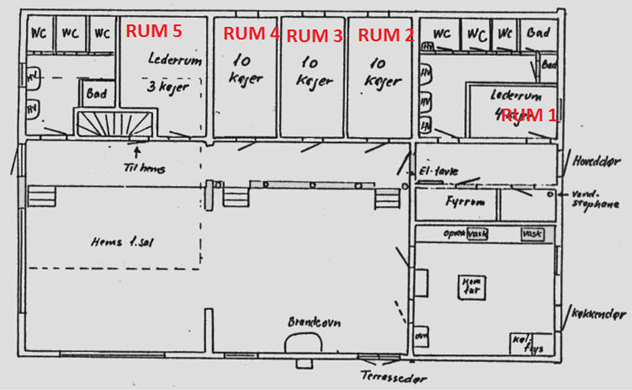
\includegraphics[width=1\linewidth]{diverse/Polarhytten_Grundplan.png}
\end{center}

\begin{tabular}{|l|l|}
\hline
%
\Norder                         &       Rum 4   \\ \hline
\Bad                            &       Rum 3   \\ \hline
\Hippier                        &       Rum 2   \\ \hline
\Alternative                    &       Hems    \\ \hline
\Poppere                        &       Hems    \\ \hline
\Fransk                         &       Hems    \\ \hline
                                &               \\ \hline
\KABS + Fulde vektorer          &       Rum 5   \\ \hline
\Hyttebombz{} + Ansvarsvektorer &       Rum 1   \\ 
%
\hline
\end{tabular}
\section{Natløb}
\begin{tabular}{L{8cm} L{8cm}}
\textbf{Menneske Torpedo}           & \textbf{Jorden er giftig - Mælkekasser}   \\
Antal: 2 hold                       & Antal: 1 hold                             \\
Ansvarlig: \Gabriel                 & Ansvarlig: \Johnny                        \\
                                    &                                           \\
\textbf{Sæd-stafet}                 & \textbf{Pik mod drøbel (kropsdele på jord)}\\
Antal: 2 hold                       & Antal: 1 hold                              \\
Ansvarlig: \Lucyfar                        & Ansvarlig: \KABS                     \\
                                    &                                             \\
\textbf{Død stjernefisk}            & \textbf{Futtog - Mad/øl - Køkkenet}         \\
Antal: 1 hold                       & Antal: 1 hold                                 \\
Ansvarlig: \Ora                     & Ansvarlig: \Hyttebombz{}                       \\
\end{tabular}

\makebox[\textwidth][c]{
\begin{tabular}{ | c | c | c | c | c | c | c |   }
\hline
	Tid & Post 1 & Post 2 & Post 3 & Post 4 & Post 5 & Post 6 \\ \hline
	21:00 & \doublecell{\Hippier \\ \Norder   }  &  & \Fransk  & \Alternative & \Bad & \Poppere \\ \hline
	21:15 & \doublecell{\Bad \\ \Poppere}        &  & \Norder  & \Hippier & \Fransk & \Alternative \\ \hline
	21:30 & \doublecell{\Alternative \\ \Fransk} &  & \Poppere & \Bad & \Norder & \Hippier \\ \hline 
	21:45 &  & \doublecell{\Hippier \\ \Poppere} & \Bad        & \Norder & \Alternative & \Fransk \\ \hline
	22:00 &  & \doublecell{\Norder \\ \Fransk}   & \Alternative & \Poppere & \Hippier & \Bad \\ \hline
	22:15 &  & \doublecell{\Bad \\ \Alternative} & \Hippier    & \Fransk & \Poppere & \Norder \\ \hline
\end{tabular}
}

\subsection{Pointskema}
\begin{tabular}{ | l | l | l | l | l | l | }
\hline
	 & Samarbejde & Engagement & Awesomeness & Præstation & Bestikkelse \\ \hline
	\Hippier &  &  &  &  &  \\ \hline
	\Norder &  &  &  &  &  \\ \hline
	\Bad &  &  &  &  &  \\ \hline
	\Poppere &  &  &  &  &  \\ \hline
	\Alternative &  &  &  &  &  \\ \hline
	\Fransk &  &  &  &  &  \\ \hline
\end{tabular}

\newpage

\subsection{Poster}
\subsubsection{Post 1 - Menneske torpedo}
Ansvarlig:	\Gabriel eller \Lucyfar\\
Sted: Bakken \\
Antal: 2 hold \\\\
\textbf{Historie:}\\
Starfish High brænder, så du og dine med studerende skal ud af bygningen hurtigst muligt. Men på vejen er der nogle flasker med ekstra ilt der skal væltes. Den bagerste person er den eneste der kan se, og skal således guide de andre russer ud af bygningen, uden at kommunikere med dem mundtligt.\\\\
\textbf{Legen:}
Russerne stiller sig på en lang række, og holder hinanden på skuldrene. De forreste for bind for øjnene, så kun den bagerste person i rækken kan se. Denne person guider nu, med slag på skuldrene de andre russer i retning af ”ilt-flaskerne”, således at de vælter.\\\\
Der gives point for antallet af væltede ``ilt-flasker'', samarbejdet, kreativiteten samt bestikkelse. Og ja, det kommer til at tælle med i den endelige karakter.\\\\
\textbf{Materialer:}

\begin{multicols}{2}
\begin{itemize}
\item 10 tomme ølflasker
\item 20 bind (til øjnene)
\end{itemize}
\end{multicols}

\textbf{Rotationsskema for post 1:}\\
\begin{tabular}{ | l | }
\hline
	 \Hippier sendes videre til post 4, \Johnny på parkeringspladsen \\ \hline
	 \Norder sendes videre til post 3, \Ora på terrassen \\ \hline
	 \Bad sendes videre til post 4, \Johnny på parkeringspladsen \\ \hline
	 \Poppere sendes videre til post 3, \Ora på terrassen \\ \hline
	 \Alternative sendes videre til post 5, \KABS i Pejsestuen \\ \hline
	 \Fransk sendes videre til post 6, \Hyttebombz{} i køkkenet \\ \hline
\end{tabular}

\newpage

\subsubsection{Post 2 - Sæd-stafet}
Ansvarlig: 	\Lucyfar eller \Gabriel\\
Sted: Bakken \\
Antal: 2 hold \\\\
\textbf{Legen:}\\
I morgen er det \#PromNight og derfor vil det være en god idé at kunne håndtere forskellige typer væsker.
Ved I hvad denne type væske hedder \#LegMedSæden \#NåNej det er en newtonisk væske... \#DTU$<$3.

Sædstafetten går ud på at transportere alt sæden fra den ene skål til den anden vha. nogle plastickrus. Man skal naturligvis bruge munden \#Høhø, og man skal så hælde sæden fra den ene kop til den næste indtil man når den anden skål. Det går ud på at tømme sin egen skål så hurtigt som muligt.\\\\
Der gives point for stil, engagement, præstation og awesomeness. Og ja, det kommer til at tælle med i den endelige karakter.\\\\
\textbf{Materialer:}
\begin{multicols}{2}
\begin{itemize}
\item 4 gryder/skåle
\item 100 plastiskkrus
\item Vand i store mængder
\item 2 x kartoffelmel
\item Stor ske
\end{itemize}
\end{multicols}

\textbf{Rotationsskema for post 2:}\\
\begin{tabular}{ | l | }
\hline
	 \Hippier sendes videre til post 5, \KABS i Pejsestuen \\ \hline
	 \Poppere sendes videre til post 4, \Johnny på parkeringspladsen \\ \hline
	 \Norder sendes videre til post 6, \Hyttebombz{} i køkkenet \\ \hline
	 \Fransk sendes videre til post 4, \Johnny på parkeringspladsen \\ \hline
\end{tabular}



\subsubsection{Post 3 - Død stjernefisk}
Ansvarlig: \Ora \\
Sted: Terrasse\\
Antal: 1 hold\\\\
\textbf{Historie:}\\
Idrætshallens fundament er sunket grundet dårligt ingeniørarbejde, er øl, cider og sodavand fra opbevaringsrummet faldet ned, og dette må under ingen omstændigheder gå til spilde. Derfor skal I nu drikke alt det i overhovedet kan, uden at falde ned i hullet. \\\\
\textbf{Legen:}\\
Et afskærmet område 1x2 meter med en skål placeret i midten illustrer et hul i fundamentet,
Russerne vælger nu en der får et sugerør og skal drikke så meget som muligt fra skålen, uden
at røre området. Hjælperne holder russen, og ingen må betræde området. \\\\
Der giver point for antal flasker der drikkes, samarbejdet, kreativiteten og bestikkelse. 
Og ja, det kommer til at tælle med i den endelige karakter.\\\\
\textbf{Materialer:}
\begin{multicols}{2}
\begin{itemize}
\item 1 skål
\item 100 sugerør
\item Gaffetape
\item Vand
\end{itemize}
\end{multicols}

\textbf{Rotationsskema for post 3:}\\
\begin{tabular}{ | l | }
\hline
	 \Fransk sendes videre til post 5, \KABS i Pejsestuen \\ \hline
	 \Norder sendes videre til post 5, \KABS i Pejsestuen \\ \hline
	 \Poppere sendes videre til post 2, \Lucyfar og \Gabriel på bakken \\ \hline
	 \Bad sendes videre til post 6, \Hyttebombz{} i køkkenet \\ \hline
	 \Alternative sendes videre til post 2, \Lucyfar og \Gabriel på bakken \\ \hline
\end{tabular}



\subsubsection{Post 4 - Jorden er giftig (Mælkekasser)}
Ansvarlig:	\Johnny \\
Sted: Parkeringsplads \\
Antal: 1 hold \\\\
\textbf{Legen:}\\
Det er snart prom night, og da vi er landet ude på ødemarken i stedet for på vores fine skole, kan I risikere, at I skal igennem en masse mudder og græs for at komme til festsalen, og vi kan jo ikke have, at det fine tøj bliver ødelagt. Derfor skal I nu øve jer på at bevæge jer uden at røre jorden. Vi har de her mælkekasser, som vi skal bruge, og det er vigtigt, at alle kommer med.
Derfor skal I gå en rute (rundt om en tom ølflaske eller forbi et kendetegn eller noget) uden at røre jorden. \\\\
Der bliver givet point for stil, engagement, præstation og awesomeness. Og ja, det kommer til at tælle med i den endelige karakter.\\\\
\textbf{Materialer:}
\begin{multicols}{2}
\begin{itemize}
\item 4 mælke-/ølkasser
\item \#EnKæmpeFest!!!
\end{itemize}
\end{multicols}

\textbf{Rotationsskema for post 4:}\\
\begin{tabular}{ | l | }
\hline
	 \Alternative sendes videre til post 6, \Hyttebombz{} i køkkenet \\ \hline
	 \Hippier sendes videre til post 6, \Hyttebombz{} i køkkenet \\ \hline
	 \Bad sendes videre til post 3, \Ora på terrassen \\ \hline
	 \Norder sendes videre til post 2, \Lucyfar og \Gabriel på bakken \\ \hline
	 \Poppere sendes videre til post 5, \KABS i Pejsestuen \\ \hline
\end{tabular}



\subsubsection{Post 5 - Pik mod drøbel (kropsdel på jord)}
Ansvarlig: \KABS \\
Sted: Pejsestuen \\
Antal: 1 hold \\\\
\textbf{Legen:}\\
Nu er det \#LateNight idrætstime, og nattens tema er at lære at strække sig og stå i usædvanlige positioner for at styrke de statiske muskler og led. Måden det foregår på er, at jeg trækker et kort, som symboliserer noget, I skal gøre, fx øre mod mave, og så skal i stå sådan med kortet mellem de kropsdele, der bliver nævnt. Hvis I taber kortet eller slipper positionen, har I tabt.\\\\
Der bliver givet point for stil, engagement, præstation og awesomeness. Og ja, det kommer til at tælle med i den endelige karakter.\\\\
\textbf{Materialer:}
\begin{multicols}{2}
\begin{itemize}
  \item Kortspil
\end{itemize}
\end{multicols}

\textbf{Regler:}\\
\begin{tabular}{ | l | l | l | }
\hline
	Kort nr. & Kropsdel 1. person & Kropsdel 2. person \\ \hline
	Es & Hånd & Hånd \\ \hline
	2 & Røv & Røv \\ \hline
	3 & Hoved & Mave \\ \hline
	4 & Hånd & Røv \\ \hline
	5 & Albue & Skulder \\ \hline
	6 & Hånd & Hår \\ \hline
	7 & Kind & Skulder \\ \hline
	8 & Pande & Pande \\ \hline
	9 & Næse & Bryst \\ \hline
	10 & Mund & Hånd \\ \hline
	Knægt & Mund & Kind \\ \hline
	Dame & Lår & Røv \\ \hline
	Konge & Fod & Øre \\ \hline
\end{tabular}

\textbf{Rotationsskema for post 5:}\\
\begin{tabular}{ | l | }
\hline
	 \Bad sendes videre til post 1, \Lucyfar og \Gabriel på bakken \\ \hline
	 \Fransk sendes videre til post 1, \Lucyfar og \Gabriel på bakken \\ \hline
	 \Norder sendes videre til post 4, \Johnny på parkeringspladsen \\ \hline
	 \Alternative sendes videre til post 3, \Ora på terrassen \\ \hline
	 \Hippier sendes videre til post 3, \Ora på terrassen \\ \hline
\end{tabular}

\newpage

\subsubsection{Post 6 - Futtog (Køkken)}
Ansvarlig: \Hyttebombz{}\\
Sted: Køkkenet\\
Antal: 1 hold\\\\
\textbf{Materialer:}
\begin{multicols}{2}
\begin{itemize}
  \item 6 roulader
  \item 6 agurker \#FlereAgurker
  \item 6 liter koldskål
  \item 6 auberginer
  \item 6 liter (billig) kakaomælk
\end{itemize}
\end{multicols}

\textbf{Rotationsskema for post 6:}\\
\begin{tabular}{ | l | }
\hline
	 \Poppere sendes videre til post 1, \Lucyfar og \Gabriel på bakken \\ \hline
	 \Alternative sendes videre til post 1, \Lucyfar og \Gabriel på bakken \\ \hline
	 \Hippier sendes videre til post 2, \Lucyfar og \Gabriel på bakken \\ \hline
	 \Fransk  sendes videre til post 2, \Lucyfar og \Gabriel på bakken \\ \hline
	 \Bad sendes videre til post 2, \Lucyfar og \Gabriel på bakken \\ \hline
\end{tabular}



\subsection{Samlet materiale liste for natløb}
\begin{multicols}{2}
\begin{itemize}
% Post 1
\item 10 tomme ølflasker
\item 20 bind (til øjnene)
% Post 2+3
\item 4+1 gryder/skåle
\item 100 plastiskkrus
\item Vand i store mængder
\item 2 x kartoffelmel
% Post 3
%1 skål
\item 100 sugerør
% Post 4
\item 4 mælke-/ølkasser
% Post 5
\item Kortspil
% Post 6
\item 6 roulader
\item 6 agurker \#FlereAgurker
\item 6 liter koldskål
\item 6 auberginer
\item 6 liter (billig) kakaomælk
\end{itemize}
\end{multicols}

\clearpage

%%%%%%%%%%%%%%  LØRDAG  %%%%%%%%%%%%%%
\section*{Lørdag}
\renewcommand{\lheadmsg}{Lørdag}
\addcontentsline{toc}{section}{Lørdag}
\section{(Sø)Stjerneløb}

\begin{tabular}{L{8cm} L{8cm}}
\textbf{Post 1}                         &  \textbf{Post 4}                              \\
PF, struktur, faglige råd og udvalg     & AUS/Studievejledningen og Fremdriftsreform    \\
Ansvarlig: \Lucyfar                     & Ansvarlig: \Ora                               \\
Sted: Rusrum 2                          & Sted: Rusrum 4                                \\
                                        &                                               \\
\textbf{Post 2}                         & \textbf{Post 5}                               \\
Kollegier, PKS og udlandsophold         & Puma                                          \\
Ansvarlig: \KABS                        & Ansvarlig: \Johnny                            \\
Sted: Rusrum 3                          & Sted: Festsalen (\#PumaUdenMusikVirkerIkk)    \\
                                        &                                               \\
\textbf{Post 3}                         & \textbf{Post 6}                               \\
Kartofler!                              & S-Huset, fredagsbarer og joints               \\
Ansvarlig: \Hyttebombz                  & Ansvarlig: \Gabriel                           \\
Sted: Terrassen/køkken                  & Sted: Hemsen                                  \\
\end{tabular}

\makebox[\textwidth][c]{
\begin{tabular}{ | l | l | l | l | l | l | l | }
\hline
	Kl        & Post 1       & Post 2        & Post 3        & Post 4        & Post 5        & Post 6 \\ \hline
	15:00     & \Hippier     & \Bad          & \Fransk       & \Norder       & \Poppere      & \Alternative \\ \hline
	15:10     & \Alternative & \Hippier      & \Bad          & \Fransk       & \Norder       & \Poppere \\ \hline
	15:20     & \Poppere     & \Alternative  & \Hippier      & \Bad          & \Fransk       & \Norder \\ \hline
	15:30     & \Norder      & \Poppere      & \Alternative  & \Hippier      & \Bad          & \Fransk \\ \hline
	15:40     & \Fransk      & \Norder       & \Poppere      & \Alternative  & \Hippier      & \Bad \\ \hline
	15:50     & \Bad         & \Fransk       & \Norder       & \Poppere      & \Alternative  & \Hippier \\ \hline
\end{tabular}
}

\subsection{Poster}
\subsubsection{Post 1}
Hvor mange har allerede meldt sig ind i PF? \#GodBeslutning

\begin{itemize}
 \item En forening af de studerende, for de studerende.
 \item En 3-dimensionel forening, der engagerer sig både Fagligt, Politisk, Socialt og på alle områder imellem.
\end{itemize}

\begin{itemize}
 \item Fagligt
 \begin{itemize}
  \item Institutstudienævn - Evaluerer kurser og undervisere, for at sikre en høj kvalitet af undervisningen.
 \end{itemize}
 \item Politisk
 \begin{itemize}
  \item Uddannelsespolitisk råd - Sidder med i blandt andet DTU's bestyrelse, og deltager i diskussioner om uddannelsespolitik, der vedrører studerende på DTU.
 \end{itemize}
 \item Socialt
 \begin{itemize}
  \item S-Huset - Mere information hos \Gabriel.
  \item Idræt og klubber - Fodbold, Badminton, Basket, Volley, Løb, Bordtennis, Dans, Klatring, Sejlads, Ølbowling, Brætspil, Foto, Poker etc. Få støtte til at oprette en ny PF klub (PF Camping?). I kommer til at møde klubberne på en rundvisning i semsteruge 3.
 \end{itemize}
 \item Rabatter
 \begin{itemize}
  \item Ulykkesforsikring, Fitness World, Lyngby Svømmehal, Briller, Aviser og meget mere...
 \end{itemize}
\end{itemize}

Aktiv i de faglige råd.

Indmelding: www.pf.dk

Spørgsmål?

\subsubsection{Post 2}
Indstilling til kollegierne sker gennem Polyteknisk Forenings IndstillingsUdvalg (PFIU).\\
Ansøgning sker gennem www.pks.nu. Fortæl lidt om de forskellige kollegier og deres barer.
\begin{multicols}{2}
\begin{itemize}
 \item Kampsaxkollegiet - Saxen (Torsdag)
 \item Andelskollegiet - placering
 \item Prof. Ostenfeldt - Nakkeosten (1. tirsdag i måneden)
 \item Willum Kann Rasmussen - VKR-Baren (Mandag, ej lovlig)
 \item William Demant - Willys vandhul (Onsdag)
 \item P.O. Pedersen - Falladen (Tirsdag og lørdag)
 \item Paul Bergsøe - Pauls Ølstue (Tirsdag og fredag)
 \item Trørød (Par og unge med børn)
 \item Nybrogård - Kældercafeen (Fredag + evt. temafest om lørdagen) - Søges gennem KAB og ikke PKS
 \item Viggo Jarls -  - Søges gennem send mail til efor@kvjf.dk.
\end{itemize}
\end{multicols}
Det meste information kan findes i rusbogen. Priser fra 2250-3300 kr.

\textbf{Udlandsophold:}\\
Rigtig mange vælger at tage et semester eller to i udlandet. Det er fedt.
\begin{itemize}
\item Skal søges et halvt til et helt år før afhængig af destination
\item DTU har aftaler med en række universiteter og sørger for SU, bolig og indskrivning hos disse
\item Søger man andre universiteter kan det gøres hos Erasmus Fonden? eller andre organisationer, så skal man selv klare ovenstående
\item Der er rigtig mange legater man kan søge - også selvom man får SU
\item Man kan få hjælp hos International Affairs i administrationen i 101
\item Praktikophold kan søges hos IAESTE (International Association for the Exchange of Students for Technical Experience)
\end{itemize}

\subsubsection{Post 3}
Skræl de kartofler!

\subsubsection{Post 4}
Afdelingen for Uddannelse og Studerende befinder sig i 101A. Alle spørgsmål om SU, dispensationer og andet kan stilles her. Desuden kan studievejledningen hjælpe med tekniske detaljer om merit, studieforløb, retningsskifte, og meget andet.
KKO, Studenterrådgivningen og Studiepræsten.

\textbf{Fremdiftsreform}\\
\begin{itemize}
  \item{Tilmelding til fag} Alle studerende \emph{skal} være tilmeldt kurser svarende til 60 \emph{nye(!)} ECTS-point hvert år (2 x 13-ugers + 3-ugers). Normalvis 30 pr. semester.
  \item{Tilmelding til prøver} ALLE studerende tilmeldes automatisk eksaminer i de fag, de er tilmeldt. Så snart eftertilmeldingsperioden er slut, kan man \emph{ikke} vælge fag om, og er i udgangspunktet forpligtet til at bestå eksamen. Hvis man dumper, skal man til reeksamen så snart man kan. Enten næste semester eller i en særlig reeksamensperiode.
  \item{Studiestartsprøve} Inden for de to første måneder afholdes en prøve som \emph{skal} bestås for at kunne fortsætte på sit studie. For jer er prøven, at I skal lægge en studieplan for hele jeres bachelor. Mere har vi ikke fået at vide.
\end{itemize}

\subsubsection*{SU}
\label{sub:SU}
\begin{itemize}
  \item{Støttetidsregler} Hvis man søger ind på en videregående uddannelse for første gang senest to år efter endt gymnasiel uddannelse, har man 12 SU-klip ud over normeret studietid. Hvis man starter mere end to år efter endt gymnasielt stuie, er man kun berettiget til SU på normeret studietid.
  \item{SU-stop} Hidtil har man kunnet være 12 måneder bagefter med studiet, før SU'en inddrages. Disse regler ændres til 6 måneder, men træder først i kraft pr. \emph{1. september 2016}.
\end{itemize}

\subsubsection{Post 5}
Dans for helvede! DAAAAAAANS!!! (Reklamér for Rusjoint).

\subsubsection{Post 6}
S-huset er placeret i bygning 101 og åbner alle hverdag kl. 7.30, senere på aftenen rykker festen fra s-huset til Kælderbaren (s-huset lukker). Kælderbaren lukker når festen er gået kold (dog senest kl. 5.00). \#HuskS-HusetPåBallerup

\textbf{Kaffestuen:} mad og drikke. Special pris på bl.a. kaffe til PF medlemmer. Åben: Man-Fre: 07:30–19:00\\
\textbf{Pejsestuen:} Hyggeområde; sofaer, poolbord og bordfodboldbord.\\
\textbf{Læsesalen:} Bagerste lokale i S-huset. Brug biblio i stedet? God til eksamensforberedelse.\\
\textbf{Kælderbaren:} Specialøl, \#Awesomeness Åben: 19:00-?? (senest 05:00)\\

\textbf{PF Caféen:} S-huset består også af PF-Caféen i bygning 306. Lige overfor der hvor I har Mat 1. Åben: Man-Fre: 07:30 – 17:00\\

\textbf{Fredagsbarer}: Åbningstider 12:00-21:00 (eller 12:00-03:00 ved lang åbning). Hegnet åbner først 14:00 pga. Kantinen.

\begin{multicols}{2}
\begin{itemize}
  \item Diagonalen - Bygn. 116
  \item Etherrummet - Bygn. 208
  \item Hegnet - Bygn. 342
  \item Maskinen - Bygn. 358
  \item Diamanten - Bygn. 414
  \item Verners Kælder - Ballerup
\end{itemize}
\end{multicols}

\textbf{Joints:}
\begin{multicols}{2}
\begin{itemize}
  \item Sensommerfest - 4. september
  \item Rusjoint - 11. september (Spiser sammen i tværgrupper - billetter ryger hurtigt)
  \item Oktoberfest - 2-3. oktober (ikke sikker)
  \item Seriøst motionsløb - 8. oktober
  \item Useriøst motionsløb - 9. oktober
  \item Julejoint - ?
  \item Julefrokost - 7. november %opdateret dato
\end{itemize}
\end{multicols}
\section{Vesteoverdragelse}
\label{sub:vaerelsefordeling}
Vestene overdrages fra \YOLO og \BIATCH til \Lucyfar og \Ora. Eventuelt skal de bunde henholdsvis øl og cocio/sodavand.

Samtidig skal russerne have at vide, at de kan skrive sig på oppyntning, barvagt, opvaskefest eller underholdning til om aftenen samt at de skal lave et vers til melodien "I en kælder sort som kul" inden aftensmaden.

Hvis man er interesseret i at hjælpe med en af de fire ting, skal man finde den vektor, der er ansvarlig for det:\\

\begin{multicols}{2}
\begin{itemize}
    \item Oprydning - \BIATCH
    \item Underholdning - \Johnny
    \item Opvaskefest - \YOLO
    \item Barvagter - \Gabriel
\end{itemize}
\end{multicols}

Der skal tages både fællesbillede og tværholdsbilleder.Russerne skal selv sørge for at samle sig i tværhold og finde fotografen \KABS 

Ellers er der cirka 3 timer, hvor de har mulighed for at skrive verset, tage et bad, tage en lur eller hvad man føler for. Desuden vil nogle af vektorerne introducere et par ølspil, man ofte støder på, på DTU (kævle, ølcrocket, ølbowling, hvad der lige er stemning for).

De har nu 5 minutter til lige at løbe ind og finde deres kostume hvis de mangler noget, og så tager vi et fællesbillede på bakken/terrassen.

\section{Festaften}
Russerne arrangerer selv festaften. Vi hænger skemaer op med tjanser i pejsestuen torsdag morgen. Dagsansvarlige annoncerer til morgenrejsning torsdag, at russerne selv skal skrive sig på.

\begin{enumerate}
\item Oppyntning - Ansvarlig: \Randildo \& \Clint
\item Bar - Ansvarlig: \Stive \& \Hemorides
\item Madlavning - Ansvarlig: \Hyttebums{Piraterne}
\item Oprydning - Ansvarlig: \Farav \& \Mighty
\item Underholdning - Ansvarlig: \Karla \& \Buddha
\end{enumerate}

\subsection*{Oppyntning - 10 russer}
\subsubsection*{Ansvar: \Randildo \& \Clint}
Dække bord, pynte borde og vægge. Der skal indkøbes:
\begin{itemize}
\item Duge
\item Balloner
\item Serpentiner
\item Fyrfadslys
\item Sølvpapir til lysestager
\item Tape
\end{itemize}

\subsection*{Bar - 10 russer}
\subsubsection*{Ansvar: \Stive \& \Hemorides}
Der bliver købt ind til 2 slags drinks. Der bliver lavet streglister så russerne betaler over ølregning individuelt. Baransvarlige skal altid være i baren, således det ikke stikker af. Fif: Vent med at blande det hele. Der skal indkøbes:
\begin{itemize}
  \item Vodka + Saftevand
  \item Rom + Cola
  \item Plastglas 400 stk.
  \item Sugerør 400 stk.
\end{itemize}

\subsection*{Madlavning - 8 russer}
\subsubsection*{Ansvar: \Hyttebums{De glade Sømænd}}
\Hyttebums{Piraterne} winger den

\subsection*{Oprydning efter aftensmad - 11 russer}
\subsubsection*{Ansvar: \Farav \& \Mighty}
Opsætning til B14s show og rengøring af Kongressen, så vi ikke behøver at gøre det fredag.\\
Almindelig oprydning og hjælp til \Hyttebums{Piraterne} i køkkenet efter maden \Hashtag{oprydningsfist}. 

\subsection*{Underholdning - 10 russer}
\subsubsection*{Ansvar: \Karla \& \Buddha}
Russerne planlægger selv aktivitet. Ideer hertil:
\begin{itemize}
  \item Sedler under tallerknerne  med ``opgaver'' under maden
  \item Et teaterstykke
  \item En dans
  \item En tale
  \item En leg - Fx en fra hvert hold skal stille en person
  \item Gæt og grimasser \Hashtag{GørNogetUpassende}
\end{itemize}

\subsection{Afsløring af Tip en Vektor}

\begin{table}[H]
\centering
\begin{tabu}{L{11.7cm} L{3.5cm}}\specialrule{1pt}{0pt}{2pt}
\rowfont{\bfseries} Spørgsmål & Svar \\ \specialrule{1pt}{2pt}{1pt}
1) Hvem valgte at bunde en masse Fernet Branca, hvorefter personen teleportede sig fra Rødby til et poolbord i S-huset? & \hemorides \\ \specialrule{.25pt}{1pt}{1pt}
2) Hvem har brugt over 300 euro på sit kostume? & \mighty \\ \specialrule{.25pt}{1pt}{1pt}
3) Hvem gemte sig under klapsæderne i 35 min. i et tog for at spare penge? & \farav \\ \specialrule{.25pt}{1pt}{1pt}
4) Hvem har sovet udenfor DTU-skiltet efter en aften i kælderbaren og herremiddag, uden at kunne huske det dagen efter? & \buddha \\ \specialrule{.25pt}{1pt}{1pt}
5) Hvem har haft blå mærker hele vejen op ad begge ben fordi personen kravlede i bjælker på forberedelsestur? & \karla \\ \specialrule{.25pt}{1pt}{1pt}
6) Hvem har snavet samtlige af sine retningsvektorer? & \randildo \\ \specialrule{.25pt}{1pt}{1pt}
7) ”Hvad?! Jeg har aldrig gjort noget dumt” & \Hyttebums{Elizabeth} \\ \specialrule{.25pt}{1pt}{1pt}
8) Hvem stod af natbussen for at kaste op, for dernæst at erfare, der ikke kom flere busser? & \clint \\ \specialrule{.25pt}{1pt}{1pt}
9) Hvem har de korteste shorts? & \clint \\ \specialrule{.25pt}{1pt}{1pt}
10) Hvem valgte at tage en en-mands brandert i Minttu på forberedelsesturen? & \Hyttebums{Turn-On} \\ \specialrule{.25pt}{1pt}{1pt}
11) Hvem valgte at kalde max. 2 stykker tøj en aften på forberedelsesturen? & \Hyttebums{Swallows} \\ \specialrule{.25pt}{1pt}{1pt}
12) Hvem kan åbne svælget og bunde hurtigst? & \stive \\ \specialrule{.25pt}{1pt}{1pt}
13) Hvem er bedst til at spule på kommando? & \buddha \\ \specialrule{.25pt}{1pt}{1pt}
14) Hvis bare røv blev spanket i kælderbaren? & \stive \\ \specialrule{.25pt}{1pt}{1pt}
15) Hvem er bedst til kiks? & \karla \\ \specialrule{.25pt}{1pt}{1pt}
16) Hvis lægge vejer, ifølge ham selv, 40kg tilsammen? & \mighty \\ \specialrule{.25pt}{1pt}{1pt}
17) Hvem er bange for fødder? & \Hyttebums{Turn-On} \\ \specialrule{.25pt}{1pt}{1pt}
18) Hvem er den bedste morgen-boller? & \Hyttebums{Turn-On} \\ \specialrule{.25pt}{1pt}{1pt}
19) Hvilket hold vandt RISK på forberedelsesturen? & \farav, \buddha, \randildo \& \clint \\ \specialrule{.25pt}{1pt}{1pt}
20) Hvem spulede ikke på RISK-aften på forberedelsesturen? & \buddha \\ \specialrule{.25pt}{1pt}{1pt}
21) Hvem blev gagget af en gærpenis? & \stive \\ \specialrule{.25pt}{1pt}{1pt}
22) Hvem kan ikke finde ud af alfabetet? & \hemorides \\ \specialrule{.25pt}{1pt}{1pt}
23) Hvem blandt vektorerne/hyttebumZ/KABS er holdets spassere? & \hemorides \& \mighty \\ \specialrule{1pt}{1pt}{0pt}
\end{tabu}
\end{table}

\clearpage

%%%%%%%%%%%%%%  SØNDAG  %%%%%%%%%%%%%%
\section*{Søndag}
\renewcommand{\lheadmsg}{Søndag}
\addcontentsline{toc}{section}{Søndag}
%%%%%%%%%%%%%%%%%%%%%%%%%%%%%%%%%%%%%%%%%%%%%%%%%%%%%%%%%%%%%%%%
%
% Alle må ændre/slette/tilføje til denne liste
%
%%%%%%%%%%%%%%%%%%%%%%%%%%%%%%%%%%%%%%%%%%%%%%%%%%%%%%%%%%%%%%%%

\section{Rengøring}
\textbf{Brug ``hyttelisten'' som tjekliste}\\
Dagsansvarlig sidder midt i festsalen \textit{(på teressen hvis godt vejr)} og tjekker af når områderne meldes godkendt af deres vektorer. Alle vektorer spørger Dagsansvarlig om lov, inden de gør noget! 
Vektoerer er 'runners', på nær øl-ansvarlig, som tæller øl!

\begin{center}
\begin{tabular}{|l|l|}\specialrule{1pt}{2pt}{0pt}
\textbf{Navn}                       &   \textbf{Ansvarsområde}               \\
\specialrule{1pt}{2pt}{0pt}
\KABS                               &   Udendørsareal (Stjæl \Lucyfar russer)\\ \hline
\Lucyfar                            &   Øl- \& kørselsansvarlig              \\ \hline
\Johnny                             &   Dametoilet                           \\ \hline
\BIATCH                             &   Værelse 1, 2, 3, 4, 5                \\ \hline
\YOLO                               &   Herretoilet                          \\ \hline
\Ora                                &   Dagsansvarlig                        \\ \hline
\Gabriel                            &   Festsale \& hems                     \\ \hline
\Hyttebombz{}                       &   Køkken (Stjæl \Ora russer)           \\ \specialrule{1pt}{2pt}{0pt}
\end{tabular}
\end{center}
\textbf{Aktivering af overflødige russer under rengøring}:\\
Det er ikke sikkert alle områder kræver lige mange russer! Når man kan se at nogle af ens russer er dovne dræn, eller der bare ikke lige er brug for dem, sender man dem ud til \KABS, på udendørsarealet, hvor de bliver sat i gang. (Husk at informere Dagsansvarlig)\\ 
Skal man bruge flere russer til div. opgaver, hentes disse fra \KABS.
Vektorer stiller sig til rådighed for \KABS når ens område er blevet rengjort.


\subsection{Køkken}
\textbf{Ansvarlig: \Hyttebombz}
\begin{multicols}{2}
\begin{enumerate}
  \item Fjern affald
  \item Sæt møbler/køkkenredskaber på plads
  \item Vask overflader (grundigt)
  \item Vask skabe
  \item Tjek/rengør opvaskemaskine
  \item Fej og vask gulvet (lige inden afgang)
\end{enumerate}
\end{multicols}

\subsection{Herretoilet}
\textbf{Ansvarlig: \YOLO}\\
\hilight{\textbf{OBS: Lad ét toilet være til brug og gør dette rent lige før afgang}}
\begin{multicols}{2}
\begin{enumerate}
  \item Fjern affald (hår, skrald mm.)
  \item Rengør håndvaske og brusekabiner
  \item Rengør og aftør toiletter
  \item Fej og vask gulvet
\end{enumerate}
\end{multicols}

\subsection{Dametoilet}
\textbf{Ansvarlig: \Johnny}
\begin{multicols}{2}
\begin{enumerate}
  \item Fjern affald (hår, skrald mm.)
  \item Rengør håndvaske og brusekabiner
  \item Rengør og aftør toiletter
  \item Fej og vask gulvet
\end{enumerate}
\end{multicols}

\subsection{Festsal \& hems}
\textbf{Ansvarlig: \Gabriel}
\begin{multicols}{2}
\begin{enumerate}
  \item Fjern affald
  \item Sæt møbler på plads
  \item Fej og vask gulvet grundigt (og én gang til lige inden afgang)
\end{enumerate}
\end{multicols}

\subsection{Værelse 1, 2, 3, 4, 5}
\textbf{Ansvarlig: \BIATCH}
\begin{multicols}{2}
\begin{enumerate}
  \item Fjern affald
  \item Fjern ting og madresser
  \item Fej og vask gulvet
\end{enumerate}
\end{multicols}

\subsection{Udendørsareal}
\textbf{Ansvarlig: \KABS}
\begin{multicols}{2}
\begin{enumerate}
  \item Fjern affald
  \item Sæt evt. møbler/ting på plads
\end{enumerate}
\end{multicols}


\section{Pizzabestilling}
\textbf{Eda's Pizzaria}\\
Lyngbygårdsvej 100\\
2800 Kgs. Lyngby\\

Tlf: 45875754\\

\textbf{Der er aftalt 45,- pr. pizza}\\
\textit{Vi tager 50,- for dem, og giver en sejere julefrokost i stedet.}\\
Ring ca. 1 time før! Dvs så hurtigt som muligt efter busafgang.\\

4 typer pizzaer:\\
- \textbf{Nr. 2, Skinke:} Tomat, ost \& skinke\\
- \textbf{Nr. 2A, Pepperoni:} Tomat, ost \& pepperoni\\
- \textbf{Nr. 202, Salat:} Tomat, ost, kødstrimler, salat \& dressing\\
- \textbf{Nr. 9, Vegetar:} Tomat, ost, champignon, paprika, ananas, asparges \& løg\\


%%%%%%%%%%%%%%  GENERALT/ANDET  %%%%%%%%%%%%%%
\section{Hvem kan hvad?}
\begin{table}[ht]
\centering
\begin{tabu}{ | l | C{2.2em} | C{2.4em} | C{2.2em} | C{3.8em} | C{2.2em} | C{2.6em} | C{2.6em} | C{3em} | c | } % | l *{9}{|C{2.8em}} |
\hline
\backslashbox{Hvem}{Hvad} & Blod & Bræk & Lort & Voldsom skade & Tale & Stille Rus & Ældre Rus & \multicolumn{2}{|c|}{\doublecell{Konflikt \\ Fysisk / Håndtering }}               \\ \hline
%    NAVN       BLOD            BRÆK            LORT    VOLDSOM SKADE   TALE        STILLE RUS   ÆLDRE RUS   KONFLIKT-Håndtering/Fysisk
     \KABS    & \cellgreen  & \cellgreen  & \cellgreen & \cellgreen  & \cellgreen & \cellgreen & \cellgreen  & \cellgreen  & \cellgreen \\ \hline
     \Lucyfar & \cellyellow & \cellgreen  & \cellgreen & \cellyellow & \cellgreen & \cellgreen & \cellyellow & \cellgreen  & \cellgreen \\ \hline
     \YOLO    & \cellgreen  & \cellgreen  & \cellgreen & \cellgreen  & \cellgreen & \cellgreen & \cellgreen  & \cellgreen  & \cellgreen \\ \hline
     \BIATCH  & \cellgreen  & \cellyellow & \cellred   & \cellgreen  & \cellgreen & \cellgreen & \cellyellow & \cellyellow & \cellred   \\ \hline
     \Johnny  & \cellgreen  & \cellgreen  & \cellgreen & \cellgreen  & \cellgreen & \cellgreen & \cellyellow & \cellyellow & \cellyellow\\ \hline
     \Ora     & \cellyellow & \cellred    & \cellred   & \cellred    & \cellgreen & \cellgreen & \cellyellow & \cellgreen  & \cellyellow\\ \hline
     \Gabriel & \cellgreen  & \cellgreen  & \cellgreen & \cellgreen  & \cellgreen & \cellgreen & \cellyellow & \cellyellow & \cellyellow\\ \hline
\Hyttebombz{A}& \cellgreen  & \cellred    & \cellred   & \cellgreen  & \cellgreen & \cellyellow& \cellgreen  & \cellgreen  & \cellyellow\\ \hline
\Hyttebombz{B}& \cellyellow & \cellgreen  & \cellgreen & \cellred    & \cellgreen & \cellgreen & \cellgreen  & \cellgreen  & \cellyellow\\ \hline
\Hyttebombz{C}& \cellgreen  & \cellyellow & \cellred   & \cellred    & \cellred   & \cellgreen & \cellyellow & \cellgreen  & \cellyellow\\ \hline
\end{tabu}
%\caption{Hvem kan hvad.}
\label{tab:hvem_kan_hvad}
\end{table}

\section{Morgenrejsning}
\begin{table}[ht]
\centering
\begin{tabu}{ | r c c c | }
\hline
\textbf{Lørdag} & Sommartider  & Space Invaders   & Tunak Tunak Tun \\ \hline
                & \KABS        & \Lucyfar \Johnny & \Gabriel \\ \hline \hline
\textbf{Søndag} & Witch Doctor & Puma             & Dub-I-Dub \\ \hline
                & \BIATCH \YOLO & \Ora \Gabriel   & \KABS \Johnny \\ \hline
\end{tabu}
\label{tab:morgenrejsning}
\end{table}

\textbf{Sange}:\\
Sommartider -- Vasco Millboy\\
Space Invaders -- Hit'n'Hide\\
Tunak Tunak Tun -- Daler Mehndi\\
Witch Doctor -- Cartoons\\
Puma -- Ruben \& Knud\\
Dub-I-Dub -- Me \& My\\


\renewcommand{\lheadmsg}{Party}

\section{Tip en Vektor - Svar}
\begin{tabular}{ | p{0.5cm} | p{7cm} | p{2cm} | p{2cm} | p{2.3cm} | }
\hline
	Nr. &  & 1 & X & 2 \\ \hline
	1 & Hvem er bedre kendt som Fernet-kongen? & Johnny DD & \colorbox{Yellow}{Lucyfar}  & Gabirel \\ \hline
	2 & Hvem har uden tvang taget fire ufrivillige bade i træk i et forsøg på at rengøre et toilet? & YOLO & Mamma Mos & \colorbox{yellow}{Ora}   \\ \hline
	3 & Hvilke to personer har tisset over kors? & \colorbox{yellow}{BIATCH} \colorbox{yellow}{ \& Gabriel} & Johnny DD \& Lucyfar & BIATCH \& Ora \\ \hline
	4 & Hvem har løbet rundt om 101 iført intet andet end en lyserød cowboyhat? & Anal Angel & Johnny DD & \colorbox{yellow}{Mamma Mos} \\ \hline
	5 & Hvem har til et vektormøde været iført intet andet end en Crocs? & Bonnie Bootay & \colorbox{yellow}{YOLO} & Lucyfar \\ \hline
	6 & Hvem har snacket med én ud af to RUC’ere på OPtur (300 deltagere)? & Gabriel & \colorbox{yellow}{BIATCH} & Ora   \\ \hline
	7 & Hvem er stjernen i den virale Flyve-Keld video på Youtube? & \colorbox{yellow}{Johnny DD} & Lucyfar & YOLO \\ \hline
	8 & Hvem har snacket med mere end 25 personer på samme aften iført et keglekostume? & Cutie Cunt & Ora   & \colorbox{yellow}{Gabriel} \\ \hline
	9 & Hvem har 4 realz mødt Elijah Wood (Frodo) på Distortion? & \colorbox{yellow}{Cutie Cunt} & Mamma Mos & Anal Angel \\ \hline
	10 & Hvem er efter en vild fredag blev kørt af sin gamle hyttebumz fra bygning 101 til Kampsax (297 meter) for at vågne op fuldstændig nøgen på et kollegieværelse, personen ikke vidste hvis var? & YOLO & \colorbox{yellow}{Ora}   & Gabriel \\ \hline
	11 & Hvem tog to kasser og tre poser pant (ca. 140 kr.) med fra Sjælland til Fyn for at pante det? & \colorbox{yellow}{Bonnie} \colorbox{yellow}{ Bootay} & Anal Angel & Gabriel \\ \hline
	12 & Hvem har kastet sit TV ud fra 3. Sal? & YOLO & BIATCH & \colorbox{yellow}{Anal Angel} \\ \hline
	13 & Hvilken sang er alle personer på holdets yndlingssang? & \colorbox{yellow}{Den nye} \colorbox{yellow}{ med Taylor} & Den gamle med Taylor & Den mellem med Taylor \\ \hline
\end{tabular}

\clearpage
\begin{multicols}{2}
[\section*{Den nye med Taylor}]
It feels like a perfect night to dress up like hipsters\\
And make fun of our exes, uh uh, uh uh.\\
It feels like a perfect night for breakfast at midnight\\
To fall in love with strangers, uh uh, uh uh.

Yeah,\\
We're happy, free, confused, and lonely at the same time\\
It's miserable and magical.\\
Oh, yeah\\
Tonight's the night when we forget about the deadlines\\
It's time

Uh oh!\\
I don't know about you\\
But I'm feeling 22\\
Everything will be alright\\
If you keep me next to you\\
You don't know about me\\
But I'll bet you want to\\
Everything will be alright\\
If we just keep dancing like we're\\
22, ooh-ooh\\
22, ooh-ooh

It seems like one of those nights,\\
This place is too crowded.\\
Too many cool kids, uh uh, uh uh (who's Taylor Swift anyway, ew?)\\
It seems like one of those nights,\\
We ditch the whole scene and end up dreaming\\
Instead of sleeping.

Yeah,\\
We're happy, free, confused, and lonely in the best way\\
It's miserable and magical.\\
Oh, yeah\\
Tonight's the night when we forget about the heartbreaks\\
It's time

Uh oh! (hey!)\\
I don't know about you\\
But I'm feeling 22\\
Everything will be alright\\
If you keep me next to you\\
You don't know about me\\
But I'll bet you want to\\
Everything will be alright (alright)\\
If we just keep dancing like we're\\
22, ooh-ooh (oh, oh, oh)\\
22, ooh-ooh\\
I don't know about you\\
22, ooh-ooh\\
22, ooh-ooh

It feels like one of those nights,\\
We ditch the whole scene.\\
It feels like one of those nights,\\
We won't be sleeping.\\
It feels like one of those nights,\\
You look like bad news.\\
I gotta have you,\\
I gotta have you.

Ooh-ooh\\
Ooh-ooh, ye-e-e-e-eah, hey\\
I don't know about you (I don't know about you)\\
But I'm feeling 22\\
Everything will be alright\\
If you keep me next to you\\
You don't know about me (you don't know about me)\\
But I'll bet you want to\\
Everything will be alright\\
If we just keep dancing like we're\\
22, ooh-ooh\\
22, ooh-ooh\\
22, ooh-ooh, yeah, yeah\\
22, ooh-ooh, yeah, yeah, yeah

It feels like one of those nights,\\
We ditch the whole scene\\
It feels like one of those nights,\\
We won't be sleeping\\
It feels like one of those nights,\\
You look like bad news,\\
I gotta have you,\\
I gotta have you.
\end{multicols}
\clearpage
\begin{table}
\addcontentsline{toc}{section}{Kontaktoplysninger}
\centering
\small
\makebox[1\textwidth][c]{%
\begin{tabu}{c L{6cm} r l R{5em}}
\specialrule{1pt}{0pt}{2pt}
\rowfont{\bfseries}
$\boxtimes$ & Navn & Mobil & Kontakt & Nummer \\
\specialrule{1pt}{2pt}{2pt}
$\square$ & Asbjørn Bastian XXXXXX (BygIn)  & 5356xxxx &                       &   \\
$\square$ & August XXXXX (BygTek)         & 5381xxxx &                       &   \\
$\square$ & Anne XXXXXXXXXX (ElTek) & 2217xxxx &                       &   \\
$\square$ & Anastasia XXXXXXXXX (TBM)   & 5362xxxx &                       &   \\
$\square$ & Andreas XXXXXXXXXXX (Eksp)    & 6016xxxx & Jens M \& Tina xxx   & 2991xxxx  \\
$\square$ & Aske Lykke XXXXXX (Prod)            & 4277xxxx & Laura B \& Hanna      & 2369xxxx  \\
$\square$ & Andreas XXXXX (PorIn)        & 2840xxxx &                       &   \\
$\square$ & Benjamin XXXXXXXXXX (Prod)   & 3055xxxx &                       &   \\
$\square$ & Brian XXXXXXX (Soft)            & 2369xxxx &                       &   \\
$\square$ & Camilla XXXXXXXX (MatTek)    & 2095xxxx &                       &   \\
$\square$ & Cæcilie XXXXXXX (Me\&Tek)          & 2012xxxx &                       &   \\
$\square$ & Christoffer F XXXXXXX (Maskin)  & 2287xxxx &                       &   \\
$\square$ & Casper XXXXXX (Soft)             & 2668xxxx &                       &   \\
$\square$ & Charlie Bo XXXXXXX (BygDes)   & 2021xxxx & Maria xxx         & 3024xxxx  \\
$\square$ & Casper Bent XXXXXXX (BygDes)  &          & Maria xxx         & 3024xxxx  \\
$\square$ & Dan Skovgaard XXXXX (De\&Inn)      & 6053xxxx &                       &   \\
$\square$ & Emil XXXXXXXX (BygIn)                  & 2216xxxx & Kamilla E xxx       & 2221xxxx  \\
$\square$ & Emilie Brisson XXXXXX (BygDes)   & 2679xxxx & Carsten (far)         & 2258xxxx \\
$\square$ & Emil Rømler XXXXXX (ElEn)         & 3177xxxx &                       &   \\
$\square$ & Henning Kjær XXXX (BygTek)        & 6133xxxx &                       &   \\
$\square$ & Jeppe XXXXXXXX (Prod)               & 2632xxxx &                       &   \\
$\square$ & Jamie XXXXXXX (Prokon)     & 2928xxxx &                       &   \\
$\square$ & Jesper XXXXXXXX (Maskin)                & 3061xxxx & ``Kæreste'' & 4225xxxx   \\
$\square$ & Johan Kristian XXXX (Maskin)       &          &                       &   \\
$\square$ & Kittiyaphong XXXXXX (BygDes)      & 8173xxxx &                       &   \\
$\square$ & Khaibar XXXXX (ProKon)              & 6081xxxx &                       &   \\
$\square$ & Kim Bekker XXXXXX (ProIn)        & 5359xxxx &                       &   \\
$\square$ & Kristine M. XXXXXXX (Eksp)          &          &                       &   \\
$\square$ & Lasse Hulbæk XXXXX (ProIn)         & 2941xxxx &                       &   \\
$\square$ & Lasse Friis XXXXX (ElTek)           &          &                       &   \\
$\square$ & Lars Klarskov XXXXXX (Trafik)    & 2217xxxx &                       &   \\
$\square$ & Leise Strange XXXXXX (BygDes)        & 6112xxxx &                         Dorte & 2349xxxx \\
$\square$ & Louise Otte XXXXXX (MatTek)       & 6176xxxx &                       &   \\
$\square$ & Malthe XXXXXXX (Ke\&Tek)      & +49 1577537xxxx & Rolf \#TidligHjem     & +49~1511680xxxx  \\
$\square$ & Mads XXXXXXXX (ElTek)     & 2218xxxx &                       &   \\
$\square$ & Mads Lysgaard XXXX (FødAna)       & 2992xxxx &                       &   \\
$\square$ & Morten XXXXXX (Maskin)            & 2339xxxx &                       &   \\
$\square$ & Mikkel Blach XXXXX (Soft)          & 2244xxxx & Harriet L xxx      & 2025xxxx  \\
$\square$ & Magnus E. XXXXXX (Soft)  & 2874xxxx &                       &   \\
$\square$ & Magnus XXXXXX (Soft)            & 2388xxxx & Susanne \& Michael    & 6012xxxx  \\
$\square$ & Mats XXXXXXX (BygTek)               &          &                       &   \\
$\square$ & Maria Væver XXXXXXX (De\&Inn)         & 5073xxxx & Charlie xxx         & 5042xxxx  \\
$\square$ & Oliver Pascal XXXXXX (NetIt)        & 3132xxxx &                       &   \\
$\square$ & Peter XXXXXX (Biotek)                 & 5190xxxx &                       &   \\
$\square$ & Phillip XXXXX (Eksp)                & 2297xxxx &                       &   \\
$\square$ & Raqib XXXXX (BygDes)               & 5335xxxx &                       &   \\
$\square$ & Robert Villum XXXXXX (BygIn)      & 2960xxxx &                       &   \\
$\square$ & Rasmus Aaby XXXXX (Eksp)           &          &                       &   \\
$\square$ & Rasmus XXXXXXXX (Maskin)             & 6160xxxx &                       &   \\
$\square$ & Rojan XXXXXX (BygTek)                &          & Ahmet xxx           & 4140xxxx  \\
$\square$ & Ruth Østergård XXXX (De\&Inn)     & 2216xxxx &                       &   \\
$\square$ & Sean Leon XXXX (BygIn)              & 2245xxxx &                       &   \\
$\square$ & Søren XXXXXXXX (ProKon)           & 2341xxxx &                       &   \\
$\square$ & Terese XXXX XXXX (BygDes)     & 2066xxxx & Majken xxx Sløk    & 4080xxxx  \\
$\square$ & Vevja XXXXXXXX (Trafik)          & 5057xxxx &                       &   \\
\end{tabu}}
\end{table}
%\clearpage
%\input{00-Skal_printes/SamletMateriale.tex}
%\clearpage
%\input{00-Skal_printes/TipenvektorUDENSVAR.tex}
%\clearpage

\end{document}